\chapter{OLS 的有限样本性质、正态回归与极大似然估计}
\label{ch:U04-finite}

第 3 章关于 OLS 的结论都是纯代数的，对任何数据成立。本章加入统计假设，把 $\hat\beta$ 当作随机变量，研究它在\key{任意固定样本量}下的性质：(1) 经典假设 A1--A5（及附加的同方差 A6、正态 A7）各管什么、违背后果如何；(2) 外生性下 $\hat\beta$ 条件无偏，条件方差为夹心式，同方差下化为 $\sigma^2(X'X)^{-1}$；(3) Gauss--Markov 定理：同方差下 OLS 是 BLUE，$s^2$ 无偏；(4) 再加正态：$\hat\beta$ 精确正态、$t\sim t_{n-K}$，OLS 即 MLE 并达到 Cramér--Rao 下界；(5) QMLE 与异方差下 OLS 的地位，一致性作为“最低要求”，以及外生/内生模型的全书路线图。大样本理论在第 5 章，检验在第 6 章，内生性在第 7--9 章。对应 Hansen 第 4 章（Least Squares Regression）与第 5 章（Normal Regression）。

%======================================================================
\section{经典线性回归模型的假设}\label{sec:U04-assump}

本节逐条给出经典线性回归模型的假设。每条假设都按“内容—用途—违背后果”来记：考试常问“某性质需要哪些假设”“某假设不成立会怎样”。

\subsection{假设一览与编号对照}

\subsubsection{五条基本假设与两条附加假设}

记样本为 $\{(y_i,x_i)\}_{i=1}^n$，$y_i$ 为标量，$x_i$ 为 $K\times1$ 回归元向量（通常含常数 1）。矩阵形式：$Y$ 为 $n\times1$，$X$ 为 $n\times K$（第 $i$ 行为 $x_i\T$），$u$ 为 $n\times1$ 误差向量，模型为 $Y=X\beta+u$。

\begin{center}
\small
\begin{tabularx}{\linewidth}{Lccl}
\toprule
假设内容 & 本书编号 & 另一常见编号 & Hansen 对应\\
\midrule
对参数线性 $y_i=x_i\T\beta+u_i$ & A1 & (2) & §4.4 线性回归模型\\
\iid 抽样 & A2 & (1) & §4.2 随机抽样\\
秩条件 / 识别 $\rank(X)=K$ & A3 & (3) & $Q_{xx}=\E(x_ix_i\T)>0$\\
外生性 $\E(u_i\mid x_i)=0$ & A4 & (5) & §4.4 中的 $\E[e\mid X]=0$\\
有界（四阶）矩 & A5 & (4) & 第 7 章：$\E Y^4<\infty$，$\E\|X\|^4<\infty$\\
\midrule
同方差 $\E(u_i^2\mid x_i)=\sigma^2$ & A6 & 讨论 BLUE 时附加 & §4.4 同方差线性回归模型\\
正态 $u_i\mid x_i\sim N(0,\sigma^2)$ & A7 & 讨论 MLE 时附加 & §5.5 正态回归模型\\
\bottomrule
\end{tabularx}
\captionof{table}{经典线性回归模型的假设与编号对照}
\end{center}

\subsubsection{另一种常见编号：抽样—线性—满秩—有界矩—外生}

另一种常见编号把五条假设按以下顺序排列，并在每条后面标出它“管”的事情：
\begin{enumerate}[label=(\arabic*)]
  \item \iid 抽样——违背时（聚类）改用聚类标准误；
  \item 对参数线性；
  \item 满秩条件——保证识别；
  \item 有界矩——排除离群值：$\E(y_i^4)<\infty$，$\E(x_{ik}^4)<\infty$；
  \item $\E(u_i\mid x_i)=0$——成立时称\term{外生模型}{exogenous model}，用 MLE 或 OLS 估计。
\end{enumerate}
考试可能按任一种编号提问，按内容对号即可。Hansen 把误差记为 $e$，本书记为 $u$。

\subsection{A1 对参数线性}

\subsubsection{“线性”指对 \texorpdfstring{$\beta$}{beta} 线性}

A1 为 $y_i=x_i\T\beta+u_i$。“线性”指 $y_i$ 是参数 $\beta$ 的线性函数，回归元本身可以是 $\log x$、$x^2$、交互项等非线性变换（第 3 章对参数线性一节）。A1 保证 OLS 有闭式解 $\hat\beta=(X'X)^{-1}X'Y$。

\subsubsection{违背 A1：OLS 估计的是最佳线性近似}

若真实关系对参数非线性（如 $y_i=\sin(x_i\T\beta)+u_i$），OLS 估计的是条件期望的最佳线性近似（第 2 章最佳线性预测一节），而不是结构参数 $\beta$。此时应改用\term{非线性最小二乘}{nonlinear least squares, NLS}，或在回归中加入非线性项。

\subsection{A2 \texorpdfstring{\iid}{i.i.d.} 抽样}

\subsubsection{定义：随机抽样}

\begin{defn}[随机抽样]\label{def:U04-rs}
\term{随机抽样}{random sampling}：$\{(y_i,x_i)\}_{i=1}^n$ 相互独立且同分布，即任意 $i\neq j$，$(y_i,x_i)$ 与 $(y_j,x_j)$ 独立，且都来自同一总体分布。
\end{defn}

含义：样本是总体的代表，我们借样本了解总体。例如用一个工资—教育样本，学习总体中工资与教育的关系。

\subsubsection{推论：\texorpdfstring{\iid}{i.i.d.} 加 A4 推出严格外生 \texorpdfstring{$\E(u\mid X)=0$}{E(u|X)=0}}

无偏性证明需要的是“误差对\key{全部}观测的回归元条件均值为零”，即 $\E(u\mid X)=0$。下面证明它可由 A2 与 A4 得到。记 $x_{-i}=\{x_j:j\neq i\}$。因为 $u_i=y_i-x_i\T\beta$ 是 $(y_i,x_i)$ 的函数，而 $(y_i,x_i)$ 与其他观测独立，所以 $(u_i,x_i)$ 与 $x_{-i}$ 独立。于是
\begin{align*}
\E(u_i\mid X) &= \E(u_i\mid x_i,\,x_{-i}) \why{$X$ 由 $x_1,\dots,x_n$ 组成}\\
&= \E(u_i\mid x_i) \why{$(u_i,x_i)$ 与 $x_{-i}$ 独立}\\
&= 0,\qquad i=1,\dots,n. \why{A4}
\end{align*}
把 $n$ 个分量排成向量即 $\E(u\mid X)=0$。直觉：条件于别人的 $x_j$，不提供关于 $u_i$ 的任何额外信息。

\subsubsection{违背 A2：聚类抽样与聚类稳健标准误}

同一学校的学生、同一行业的企业、同一省份的县，观测之间往往相关，这称为\term{聚类}{cluster}。此时 A2 \key{在个体层面不成立，在聚类层面成立}：同一聚类内的观测相关，不同聚类之间独立。

后果：只要外生性成立——聚类数据下需要聚类内的严格外生 $\E(u_g\mid X_g)=0$，其中 $u_g$、$X_g$ 分别为聚类 $g$ 的误差向量与回归元矩阵——$\hat\beta$ 仍无偏、一致，但\key{方差公式错误}：常规标准误通常偏小，需改用\term{聚类稳健标准误}{cluster-robust standard error}（第 5 章）。

\begin{center}
\begin{tikzpicture}[dot/.style={circle,fill=black,inner sep=0.9pt}]
\draw[blue!70,thick] (0,0) ellipse (0.95 and 0.65);
\foreach \p in {(-0.45,0.15),(0.3,0.3),(-0.15,-0.1),(0.1,-0.3),(0.5,-0.15)} \node[dot] at \p {};
\node[blue!70!black,font=\small] at (0,-1.0) {聚类 1};
\draw[red!70,thick] (2.6,0) ellipse (0.95 and 0.65);
\draw[red!70,thick] (3.9,0) ellipse (0.95 and 0.65);
\foreach \p in {(2.2,0.2),(2.6,0.35),(2.35,-0.25),(3.25,0.05),(3.0,-0.3),(4.0,0.3),(4.4,-0.1),(3.7,-0.35)} \node[dot] at \p {};
\node[red!70!black,font=\small] at (3.25,-1.0) {两个聚类重叠：相关};
\end{tikzpicture}
\captionof{figure}{聚类示意：聚类内观测相关，不同聚类之间独立；若两组相互重叠，二者也相关，应合并为同一聚类}
\end{center}

\subsubsection{易错：\texorpdfstring{\iid}{i.i.d.} 不蕴含同方差}

\begin{note}[\iid 不等于同方差]
常见错误说法：“$(y_i,x_i)$ 是 \iid 的，所以回归是同方差的。”这是错的。\iid 只说明不同个体来自同一分布；同方差要求给定 $x$ 后误差方差不随 $x$ 变。每个个体都可以有 $\Var(u_i\mid x_i)=\sigma^2(x_i)$，只要函数 $\sigma^2(\cdot)$ 对所有人相同，样本仍是 \iid 的。
\end{note}

\subsection{A3 秩条件与识别}

\subsubsection{\texorpdfstring{$\rank(X)=K$}{rank(X)=K} 等价于无完全多重共线性}

A3：$\rank(X)=K$，即 $X$ 列满秩；总体版本为 $Q_{xx}=\E(x_ix_i\T)$ 正定。它等价于 $X'X$ 可逆，也等价于回归元之间没有\term{完全多重共线性}{perfect multicollinearity}（第 3 章识别与多重共线性一节）。必要条件是 $n\ge K$。

\subsubsection{违背 A3：不可识别；近似违背：方差膨胀}

完全违背时 $X'X$ 不可逆，正规方程有无穷多解，$\hat\beta$ 不唯一，$\beta$ 不可识别。近似违背（高度共线）时 $\beta$ 仍可识别，但方差膨胀，估计很不精确（见本章“方差的决定因素”一小节）。

\subsection{A4 外生性 \texorpdfstring{$\E(u\mid x)=0$}{E(u|x)=0} 及其两个推论}

\subsubsection{定义：外生性}

\begin{defn}[外生性]\label{def:U04-exog}
\term{外生性}{exogeneity}：$\E(u_i\mid x_i)=0$，即给定回归元，误差的条件均值为零。
\end{defn}

由第 2 章 CEF 误差性质一节，A4 推出以下两条。

\subsubsection{推论 (a)：\texorpdfstring{$\E(u)=0$}{E(u)=0}——模型含截距时总能满足}

\begin{align*}
\E(u_i) &= \E\big[\E(u_i\mid x_i)\big] \why{迭代期望律}\\
&= \E[0]=0. \why{A4}
\end{align*}
推论 (a) “总能”满足，只要模型含截距。设 $y=x_1\beta_1+u$ 而 $\E(u)=a\neq0$，则
\begin{align*}
y &= x_1\beta_1+u = a+x_1\beta_1+(u-a), \why{加减常数 $a$}\\
\E(u-a) &= \E(u)-a=0. \why{新误差均值为零，$a$ 被截距吸收}
\end{align*}
所以 $\E(u)=0$ 只是对截距的“标准化”，不构成实质约束；代价是截距失去单独的经济解释。

\subsubsection{推论 (b)：\texorpdfstring{$\Cov(u,x)=0$}{Cov(u,x)=0}，\texorpdfstring{$u$}{u} 与 \texorpdfstring{$x$}{x} 不相关}

\begin{align*}
\Cov(x_i,u_i) &= \E(x_iu_i)-\E(x_i)\E(u_i) \why{协方差定义}\\
&= \E(x_iu_i) \why{推论 (a)：$\E(u_i)=0$}\\
&= \E\big[\E(x_iu_i\mid x_i)\big] \why{迭代期望律}\\
&= \E\big[x_i\,\E(u_i\mid x_i)\big] \why{条件期望中提出已知量 $x_i$}\\
&= 0. \why{A4}
\end{align*}
直观上，$y$ 的变异分成两块：$x$ 能解释的部分与 $u$ 的部分，两块互不重叠。

\begin{center}
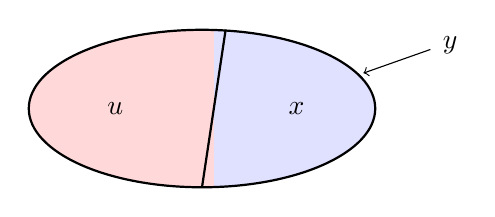
\begin{tikzpicture}
\begin{scope}
\clip (0,0) ellipse (2.2 and 1.0);
\fill[red!15] (-2.3,-1.1) rectangle (0.15,1.1);
\fill[blue!12] (0.15,-1.1) -- (0.15,1.1) -- (2.3,1.1) -- (2.3,-1.1) -- cycle;
\end{scope}
\draw[thick] (0,0) ellipse (2.2 and 1.0);
\draw[thick] (0.3,1.0) -- (0,-1.0);
\node at (-1.1,0) {$u$};
\node at (1.2,0) {$x$};
\draw[->] (2.9,0.75) -- (2.05,0.45);
\node at (3.15,0.8) {$y$};
\end{tikzpicture}
\captionof{figure}{$y$ 的变异分为 $x$ 的部分与 $u$ 的部分，两者不重叠（$\Cov(u,x)=0$）}
\end{center}

\subsubsection{反向不成立：(a)+(b) 推不出 \texorpdfstring{$\E(u\mid x)=0$}{E(u|x)=0}}

不相关比均值独立弱。反例：$x\sim N(0,1)$，$u=x^2-1$。
\begin{align*}
\E(u) &= \E(x^2)-1=1-1=0, \why{$\E(x^2)=\Var(x)=1$}\\
\Cov(x,u) &= \E(x^3)-\E(x)=0-0=0, \why{标准正态奇数阶矩为零}\\
\E(u\mid x) &= x^2-1\neq0. \why{$u$ 是 $x$ 的函数}
\end{align*}
(a)、(b) 都成立，但 A4 不成立。

\subsubsection{违背 A4：内生性}

$\E(u\mid x)\neq0$ 称为\term{内生性}{endogeneity}。此时 OLS \key{有偏且不一致}，需要 IV/2SLS/GMM（见本章路线图一节，第 7--8 章）。

\begin{note}[严格外生与同期外生]
有限样本无偏性需要\term{严格外生性}{strict exogeneity} $\E(u\mid X)=0$：误差与\key{所有}观测的回归元都均值无关。截面 \iid 下它由 $\E(u_i\mid x_i)=0$ 自动得到（见上面 A2 的推论）。但在时间序列或动态面板中，若 $x_t$ 含 $y_{t-1}$，则 $u_t$ 与未来的回归元 $x_{t+1}$（其中含 $y_t$）相关，严格外生不成立，OLS 在有限样本中有偏（但可能一致）。第 12 章动态面板的 Nickell 偏误即源于此。
\end{note}

\subsection{A5 有界矩：排除离群值}

\subsubsection{四阶矩条件：\texorpdfstring{$\E(y_i^4)<\infty$}{E(y\^4)<inf}，\texorpdfstring{$\E\|x_i\|^4<\infty$}{E||x||\^4<inf}}

A5 要求 $\E(y_i^4)<\infty$，且每个分量 $\E(x_{ik}^4)<\infty$（$k=1,\dots,K$）。Hansen 写成 $\E\|x_i\|^4<\infty$，二者等价：
\begin{align*}
\|x_i\|^4 &= \Big(\textstyle\sum_{k=1}^K x_{ik}^2\Big)^2 \le K\textstyle\sum_{k=1}^K x_{ik}^4, \why{Cauchy--Schwarz 不等式}\\
x_{ik}^4 &\le \|x_i\|^4. \why{一个分量不超过整体}
\end{align*}
取期望即知：所有 $\E(x_{ik}^4)$ 有限 $\iff$ $\E\|x_i\|^4$ 有限。一句话概括 A5：\key{有界矩 $\to$ 排除离群值}。

\subsubsection{A5 的作用：大数定律、中心极限定理与方差估计}

A5 排除了极端值频繁出现的重尾分布，使大数定律、中心极限定理以及方差估计（含 $\hat u_i^2x_ix_i\T$ 的四阶项）成立（第 5 章）。

\subsubsection{一致性只需二阶矩：A1--A5 是充分条件}

严格说，一致性只需二阶矩有限（Hansen 第 7 章的第一组假设）；四阶矩用于渐近正态与稳健方差估计的一致性。常说“在 A1--A5 下 $\hat\beta_{OLS}$ 一致”，这是充分条件而非必要条件。

\subsubsection{违背 A5：少数离群点主导估计}

违背 A5 时，少数离群点主导估计（第 3 章离群点与影响观测一节），标准误不可靠。补救：检查数据、取对数、缩尾或用稳健方法。

\subsection{假设汇总：用途、违背后果与补救}

\begin{center}
\small
\begin{tabularx}{\linewidth}{lLLL}
\toprule
假设 & 用于 & 违背的后果 & 补救\\
\midrule
A1 对参数线性 & 闭式解 & 估计的是线性近似 & NLS、加非线性项\\
A2 \iid & 严格外生、方差公式 & 方差公式错（聚类/相关） & 聚类稳健 SE（第 5 章）\\
A3 满秩 & 识别、$\hat\beta$ 存在 & 不可识别；近似违背时方差大 & 删冗余变量、增加样本\\
A4 外生 & 无偏、一致 & 有偏且不一致 & IV/2SLS/GMM（第 7--8 章）\\
A5 有界矩 & 渐近正态、方差估计 & 离群点主导、推断失效 & 查数据、缩尾、稳健方法\\
A6 同方差 & BLUE、$\sigma^2(X'X)^{-1}$ & 非有效；常规 SE 错误 & 稳健 SE；GLS/WLS\\
A7 正态 & 精确 $t$、$F$ 分布 & 小样本精确分布失效 & 用渐近分布（第 5 章）\\
\bottomrule
\end{tabularx}
\captionof{table}{各假设的用途、违背后果与补救}
\end{center}

\begin{prac}[判断违背了哪条假设]
指出下列情形分别违背哪条假设，并说明对 OLS 的后果：(a) 用全国各县数据，同一省的县受共同政策冲击；(b) 回归元同时包含“年龄”“受教育年限”和“潜在工作经验 $=$ 年龄 $-$ 教育 $-6$”；(c) 工资方程遗漏了与教育相关的能力；(d) 收入数据中有个别亿万富翁。
\answer
(a) 违背 A2：个体层面不独立，同省的县构成聚类。若外生性成立，$\hat\beta$ 仍无偏、一致，但常规标准误错误（通常偏小），应按省聚类。
(b) 违背 A3：经验 $=$ 年龄 $-$ 教育 $-6$ 与常数项、年龄、教育完全共线，$X'X$ 不可逆，三者的系数不可识别，软件会自动删去一个。
(c) 违背 A4：能力进入误差且与教育相关。OLS 有偏、不一致；若能力与工资、教育都正相关，教育回报被高估。
(d) 违背 A5：重尾、离群值。少数观测主导估计和方差，推断不可靠；应检查数据、取对数或缩尾。
\end{prac}

\begin{english}
The classical assumptions are: (A1) linearity in parameters, $y_i=x_i'\beta+u_i$; (A2) i.i.d.\ sampling; (A3) full column rank of $X$ (identification); (A4) exogeneity, $\E(u_i\mid x_i)=0$, which implies $\E(u_i)=0$ (without loss of generality when an intercept is included) and $\Cov(u_i,x_i)=0$; (A5) finite fourth moments, $\E(y_i^4)<\infty$ and $\E\|x_i\|^4<\infty$, which rules out extreme outliers. Under random sampling, A4 implies strict exogeneity $\E(u\mid X)=0$. Under clustering, A2 fails at the individual level but holds at the cluster level.
\end{english}

%======================================================================
\section{OLS 估计量的分解：\texorpdfstring{$\hat\beta=\beta+(X'X)^{-1}X'u$}{beta-hat = beta + (X'X)\^{}-1 X'u}}\label{sec:U04-decomp}

OLS 的一切有限样本与大样本性质，都从把真实模型代入 OLS 公式这一步开始。

\subsection{代入真实模型：抽样误差 \texorpdfstring{$\hat\beta-\beta=(X'X)^{-1}X'u$}{beta-hat - beta = (X'X)\^{}-1 X'u}}

要证：$\hat\beta$ 等于真值加上误差的一个线性组合。思路：把 $Y=X\beta+u$ 代入 $\hat\beta=(X'X)^{-1}X'Y$ 后展开。
\begin{align*}
\hat\beta_{OLS} &= (X'X)^{-1}X'Y \why{OLS 公式（A3 保证可逆）}\\
&= (X'X)^{-1}X'(X\beta+u) \why{代入真实模型 $Y=X\beta+u$}\\
&= (X'X)^{-1}(X'X)\beta+(X'X)^{-1}X'u \why{矩阵乘法分配律}\\
&= \beta+(X'X)^{-1}X'u. \why{$(X'X)^{-1}(X'X)=I_K$}
\end{align*}
即
\begin{equation}\label{eq:U04-decomp}
\hat\beta-\beta=(X'X)^{-1}X'u .
\end{equation}
$\hat\beta-\beta$ 称为\term{抽样误差}{sampling error}。它是误差 $u$ 的\key{线性函数}，权重矩阵 $(X'X)^{-1}X'$ 只依赖 $X$。后面求条件期望、条件方差、正态下的分布，都只是对 \eqref{eq:U04-decomp} 右边做运算。

\subsection{“分母”与“分子”：通往大样本理论的写法}

把 \eqref{eq:U04-decomp} 改写成样本均值的形式。先注意 $X'=[x_1,\dots,x_n]$（$K\times n$），所以
\begin{align*}
X'X &= \textstyle\sum_{i=1}^n x_ix_i\T, \why{分块矩阵乘法}\\
X'u &= \textstyle\sum_{i=1}^n x_iu_i. \why{分块矩阵乘法}
\end{align*}
于是
\begin{align*}
\hat\beta-\beta &= (X'X)^{-1}X'u \why{\eqref{eq:U04-decomp}}\\
&= \Big(\tfrac1n X'X\Big)^{-1}\Big(\tfrac1n X'u\Big) \why{$(cA)^{-1}=c^{-1}A^{-1}$，$n$ 与 $\tfrac1n$ 相消}\\
&= \underbrace{\Big(\frac1n\sum_{i=1}^n x_ix_i\T\Big)^{-1}}_{\text{“分母”}}\ \underbrace{\Big(\frac1n\sum_{i=1}^n x_iu_i\Big)}_{\text{“分子”}}. \why{代入上面两式}
\end{align*}
两条分析路线由此分开：
\begin{itemize}
  \item \key{有限样本分析}（本章）：条件于 $X$，“分母”是常数，对“分子”求条件期望和条件方差；
  \item \key{大样本分析}（第 5 章）：对“分母”用大数定律（$\to\E(x_ix_i\T)$），对“分子”用大数定律（$\to\E(x_iu_i)=0$，得一致性）和中心极限定理（乘 $\sqrt n$ 后渐近正态）。
\end{itemize}

\begin{english}
Substituting the true model $Y=X\beta+u$ into $\hat\beta=(X'X)^{-1}X'Y$ gives $\hat\beta=\beta+(X'X)^{-1}X'u$, so the sampling error $\hat\beta-\beta=(X'X)^{-1}X'u$ is a linear function of the errors with weights depending only on $X$. Equivalently, $\hat\beta-\beta=(n^{-1}\sum_i x_ix_i')^{-1}(n^{-1}\sum_i x_iu_i)$; finite-sample analysis conditions on $X$, while asymptotic analysis applies the law of large numbers and the central limit theorem to the two sample averages.
\end{english}

%======================================================================
\section{无偏性}\label{sec:U04-unbiased}

\subsection{定义：无偏与偏误——有限样本性质}

\begin{defn}[无偏]\label{def:U04-unbiased}
估计量 $\hat\theta$ 称为\term{无偏}{unbiased}的，若对参数空间中所有 $\theta$ 都有 $\E(\hat\theta)=\theta$。\term{偏误}{bias}定义为 $\E(\hat\theta)-\theta$。
\end{defn}

无偏性是\term{有限样本性质}{finite-sample property}：它对任何固定的样本量都可以成立，$n=1,10,20$ 都行，不需要 $n\to\infty$。

\subsubsection{无偏只保证“平均命中”：单个估计值仍需检验}

无偏说的是“重复抽样的平均”等于真值，不是说手中这一个估计值等于真值。例如算得 $\hat\beta=0.15$，它和某个假设值（如 $\beta=0$ 或 $\beta=1$）之间的差异是抽样波动还是真实差异，需要标准误与检验来判断（第 6 章）。

\subsection{OLS 的条件无偏性}

\subsubsection{定理：A1--A4 下 \texorpdfstring{$\E(\hat\beta\mid X)=\beta$}{E(beta-hat|X)=beta}}

\begin{thm}[OLS 的无偏性]\label{thm:U04-unbiased}
在 A1--A4 下（A2 用于由 A4 得到 $\E(u\mid X)=0$），
\[
\E(\hat\beta\mid X)=\beta,\qquad\text{从而}\qquad \E(\hat\beta)=\beta .
\]
（Hansen §4.5。）
\end{thm}

\subsubsection{证明：条件于 \texorpdfstring{$X$}{X} 提出常数矩阵，再用迭代期望律}

思路：对分解式 \eqref{eq:U04-decomp} 取条件期望；给定 $X$ 时权重矩阵是常数，可以提到期望外面。
\begin{align*}
\E(\hat\beta\mid X) &= \E\big[\beta+(X'X)^{-1}X'u\,\big|\,X\big] \why{分解式}\\
&= \beta+\E\big[(X'X)^{-1}X'u\,\big|\,X\big] \why{期望线性性；$\beta$ 为常数}\\
&= \beta+(X'X)^{-1}X'\,\E(u\mid X) \why{给定 $X$ 时 $(X'X)^{-1}X'$ 是常数}\\
&= \beta. \why{严格外生 $\E(u\mid X)=0$}\\
\E(\hat\beta) &= \E\big[\E(\hat\beta\mid X)\big]=\E[\beta]=\beta. \why{迭代期望律}
\end{align*}
条件无偏比无条件无偏更强：它说明无论抽到怎样的 $X$，平均而言 $\hat\beta$ 都命中 $\beta$。

\subsubsection{证明用到与没用到的假设}

\begin{itemize}
  \item \key{用到}：A1（模型形式 $Y=X\beta+u$）、A3（$(X'X)^{-1}$ 存在）、A4 与 A2（合起来给出 $\E(u\mid X)=0$）。
  \item \key{没有用到}：同方差、正态、四阶矩。所以\key{异方差下 OLS 仍无偏}。
\end{itemize}

\subsubsection{从条件无偏到无条件无偏：\texorpdfstring{$\E\|\hat\beta\|<\infty$}{E||beta-hat|| < inf} 的细节}

由 $\E(\hat\beta\mid X)=\beta$ 推出 $\E(\hat\beta)=\beta$，严格说还需要 $\E\|\hat\beta\|<\infty$。反例（Hansen §4.7）：回归元只有一个虚拟变量 $D_i$，$P(D_i=1)=p\in(0,1)$，则 $\hat\beta=\sum_iD_iy_i/\sum_iD_i$。由于
\[
P\Big(\textstyle\sum_{i=1}^nD_i=0\Big)=(1-p)^n>0,
\]
$\hat\beta$ 以正概率不存在，因而没有有限的矩。回归元连续分布时这一问题消失：Kinal (1980) 证明，若回归元与误差联合正态，则
\[
\E\|\hat\beta\|^r<\infty\iff r<n-K+1 .
\]
取 $r=1$：只要 $n-K>0$，$\E\|\hat\beta\|<\infty$，无条件无偏成立；取 $r=2$：$n-K>1$ 时无条件方差也存在。一般教材略去这一细节。

\subsection{岭回归：一个有偏的线性估计量}

\begin{prac}[岭回归的条件期望与偏误]
设 $\E(Y\mid X)=X\beta$，岭回归估计量 $\hat\beta_R=(X'X+\lambda I_K)^{-1}X'Y$，$\lambda>0$ 为固定常数。求 $\E(\hat\beta_R\mid X)$，判断是否无偏。
\answer
\begin{align*}
\E(\hat\beta_R\mid X) &= (X'X+\lambda I_K)^{-1}X'\,\E(Y\mid X) \why{给定 $X$ 时权重为常数}\\
&= (X'X+\lambda I_K)^{-1}X'X\beta. \why{$\E(Y\mid X)=X\beta$}\\
\E(\hat\beta_R\mid X)-\beta &= (X'X+\lambda I_K)^{-1}\big[X'X-(X'X+\lambda I_K)\big]\beta \why{提出 $(X'X+\lambda I_K)^{-1}$}\\
&= -\lambda(X'X+\lambda I_K)^{-1}\beta. \why{化简方括号}
\end{align*}
$\lambda>0$ 时偏误不为零（除非 $\beta=0$），所以岭回归\key{有偏}，偏误方向是把估计值向 $0$ 收缩。岭回归以偏误换取更小的方差（偏误—方差权衡）。
\end{prac}

\subsection{无偏与一致的区别}

\subsubsection{对照表}

\begin{center}
\small
\begin{tabularx}{\linewidth}{lLL}
\toprule
 & 无偏（unbiased） & 一致（consistent）\\
\midrule
定义 & $\E(\hat\theta)=\theta$ & $\hat\theta\pto\theta$（$n\to\infty$）\\
性质类型 & 有限样本（任意 $n$） & 大样本（$n\to\infty$）\\
直觉 & 重复抽样的平均命中真值 & 样本越大，估计越集中在真值附近\\
OLS 所需 & $\E(u\mid X)=0$ & $\E(x_iu_i)=0$ + 大数定律（第 5 章）\\
\bottomrule
\end{tabularx}
\captionof{table}{无偏与一致的对照}
\end{center}

\subsubsection{样本均值：既无偏又一致}

最简单的例子是样本均值（Hansen §4.3）。设 $y_1,\dots,y_n$ \iid，$\E y_i=\mu$，$\Var(y_i)=\sigma^2$。
\begin{align*}
\E(\bar y) &= \tfrac1n\textstyle\sum_{i=1}^n\E(y_i)=\mu, \why{期望线性性：无偏}\\
\Var(\bar y) &= \tfrac1{n^2}\textstyle\sum_{i=1}^n\Var(y_i)=\sigma^2/n, \why{独立，协方差项为零}\\
P(|\bar y-\mu|>\varepsilon) &\le \frac{\Var(\bar y)}{\varepsilon^2}=\frac{\sigma^2}{n\varepsilon^2}\to0. \why{Chebyshev 不等式：一致}
\end{align*}
注意 $\bar y$ 是随机的样本统计量，$\mu$ 是固定的总体参数；同理 $\frac1n\sum_ix_ix_i\T$ 是 $\E(x_ix_i\T)$ 的估计量。

\subsubsection{两种性质互不蕴含：两个反例}

\begin{itemize}
  \item \key{无偏但不一致}：用第一个观测 $\tilde\mu=y_1$ 估计 $\mu$。$\E y_1=\mu$，但 $\Var(y_1)=\sigma^2$ 不随 $n$ 减小，$\tilde\mu$ 不收敛到 $\mu$。
  \item \key{有偏但一致}：$\check\mu=\bar y+1/n$，偏误 $1/n\to0$，方差 $\sigma^2/n\to0$。误差方差的极大似然估计 $\hat\sigma^2_{MLE}=SSR/n$ 也属此类（见本章 MLE 一节）。
\end{itemize}
一致性是“有效推断的最低要求”（见本章一致性一节）。

\begin{prac}[Unbiasedness versus consistency]
Explain the difference between unbiasedness and consistency. Give an example of an estimator that is (a) unbiased but not consistent, (b) consistent but biased. Which property is called the ``minimum requirement'' for valid inference, and why?
\answer
无偏：$\E\hat\theta=\theta$，是对任意固定 $n$ 成立的有限样本性质；一致：$\hat\theta\pto\theta$，是 $n\to\infty$ 时的大样本性质。
(a) 用单个观测 $y_1$ 估计 $\mu$：无偏，但方差恒为 $\sigma^2$，不收敛。
(b) $\hat\sigma^2_{MLE}=SSR/n$：$\E(\hat\sigma^2_{MLE}\mid X)=\frac{n-K}{n}\sigma^2$，有偏，但偏误 $\to0$ 且方差 $\to0$，一致；或 $\bar y+1/n$。
一致性被称为“minimum requirement for valid inference”：不一致的估计量即使样本无限大也不会接近真值，基于它的推断没有意义；而大样本下的检验、置信区间都建立在一致性（及渐近正态）之上。
\end{prac}

\begin{english}
Under linearity, full rank and strict exogeneity $\E(u\mid X)=0$ (implied by random sampling and $\E(u_i\mid x_i)=0$), $\E(\hat\beta\mid X)=\beta+(X'X)^{-1}X'\E(u\mid X)=\beta$, and by the law of iterated expectations $\E(\hat\beta)=\beta$. Unbiasedness is a finite-sample property and does not require homoskedasticity or normality. Unbiasedness and consistency do not imply each other: $y_1$ is unbiased but inconsistent for $\mu$, while $\bar y+1/n$ is biased but consistent.
\end{english}

%======================================================================
\section{OLS 的条件方差}\label{sec:U04-var}

\subsection{一般情形：夹心式 \texorpdfstring{$(X'X)^{-1}X'\Omega X(X'X)^{-1}$}{(X'X)\^{}-1 X'Omega X (X'X)\^{}-1}}

记误差的条件协方差矩阵
\[
\Omega=\Var(u\mid X)=\E(uu'\mid X)\qquad(n\times n),
\]
第二个等号用了 $\E(u\mid X)=0$。要证：$\Var(\hat\beta\mid X)$ 是“$(X'X)^{-1}$ 夹 $X'\Omega X$”。思路：对分解式用 $\Var(Au)=A\Var(u)A'$。记 $A=(X'X)^{-1}X'$（$K\times n$），则
\begin{align*}
A' &= X\big[(X'X)^{-1}\big]' = X(X'X)^{-1}. \why{$(AB)'=B'A'$；$(X'X)^{-1}$ 对称}
\end{align*}
\begin{align*}
\Var(\hat\beta\mid X) &= \Var\big(\beta+(X'X)^{-1}X'u\,\big|\,X\big) \why{分解式}\\
&= \Var\big((X'X)^{-1}X'u\,\big|\,X\big) \why{加常数 $\beta$ 不改变方差}\\
&= (X'X)^{-1}X'\,\Var(u\mid X)\,X(X'X)^{-1} \why{$\Var(Au)=A\Var(u)A'$，给定 $X$ 时 $A$ 为常数}\\
&= (X'X)^{-1}X'\Omega X(X'X)^{-1}. \why{记 $\Omega=\Var(u\mid X)$}
\end{align*}
\begin{equation}\label{eq:U04-sandwich}
\Var(\hat\beta\mid X)=(X'X)^{-1}\,X'\Omega X\,(X'X)^{-1}.
\end{equation}
这称为\term{夹心式}{sandwich form}：两片“面包”$(X'X)^{-1}$ 夹着“肉”$X'\Omega X$。标准误是方差（的估计）的平方根：$se(\hat\beta)^2=\Var(\hat\beta)$，即 $se=\sqrt{\Var}$。

\subsection{\texorpdfstring{\iid}{i.i.d.} 异方差：\texorpdfstring{$\Omega=D=\diag(\sigma_1^2,\dots,\sigma_n^2)$}{Omega = D = diag(sigma\_i\^{}2)}}

\subsubsection{\texorpdfstring{\iid}{i.i.d.} 抽样使 \texorpdfstring{$\Omega$}{Omega} 成为对角阵}

先看非对角元（$i\neq j$）。由 A2，$(u_i,x_i)$ 与 $(u_j,x_j)$ 独立，且二者与其余观测独立：
\begin{align*}
\E(u_iu_j\mid X) &= \E(u_iu_j\mid x_i,x_j) \why{其余观测独立，不提供信息}\\
&= \E(u_i\mid x_i)\,\E(u_j\mid x_j) \why{$(u_i,x_i)$ 与 $(u_j,x_j)$ 独立}\\
&= 0. \why{A4}
\end{align*}
再看对角元：同理 $\E(u_i^2\mid X)=\E(u_i^2\mid x_i)\equiv\sigma_i^2=\sigma^2(x_i)$。所以
\[
\Omega=D=\begin{pmatrix}\sigma_1^2 & & 0\\ & \ddots & \\ 0 & & \sigma_n^2\end{pmatrix}.
\]

\subsubsection{异方差下的方差公式}

\begin{align*}
X'DX &= \textstyle\sum_{i=1}^n x_i\,\sigma_i^2\,x_i\T \why{$D$ 对角，按行展开}\\
\Var(\hat\beta\mid X) &= (X'X)^{-1}\Big(\textstyle\sum_{i=1}^n x_ix_i\T\sigma_i^2\Big)(X'X)^{-1}. \why{代入夹心式}
\end{align*}
若存在聚类，不同聚类之间独立而聚类内相关，$\Omega$ 是\key{分块对角阵}（第 5 章）。

\subsection{同方差：\texorpdfstring{$\Omega=\sigma^2I_n\Rightarrow\sigma^2(X'X)^{-1}$}{Omega = sigma\^{}2 I => sigma\^{}2 (X'X)\^{}-1}}

同方差（A6）$\Var(u_i\mid x_i)=\sigma^2$ 加上 A2 给出 $\Omega=\sigma^2I_n$：
\begin{align*}
\Var(\hat\beta\mid X) &= (X'X)^{-1}X'(\sigma^2I_n)X(X'X)^{-1} \why{代入 $\Omega=\sigma^2I_n$}\\
&= \sigma^2(X'X)^{-1}(X'X)(X'X)^{-1} \why{$\sigma^2$ 为标量，可提出}\\
&= \sigma^2(X'X)^{-1}. \why{$(X'X)^{-1}(X'X)=I_K$}
\end{align*}
在所有线性无偏估计量中，这是\key{最小的}条件方差（下界）——这正是 Gauss--Markov 定理（下一节）的内容：同方差下 OLS 是 BLUE。

异方差时 $\Omega=\diag(\sigma_1^2,\dots,\sigma_n^2)$，$\sigma^2(X'X)^{-1}$ 不再是真实方差。解决办法是\term{稳健标准误}{robust standard errors}：直接估计夹心式，
\[
\widehat\Var(\hat\beta)=(X'X)^{-1}X'\hat\Omega X(X'X)^{-1},\qquad \hat\Omega=\diag(\hat u_1^2,\dots,\hat u_n^2)
\]
（本章误差方差一节给出其有限样本形式，第 5 章详述）。

\subsection{固定设计与随机设计}

\subsubsection{固定设计：\texorpdfstring{$X$}{X} 非随机}

\term{固定设计}{fixed design}：$X$ 非随机（“$X$ is fixed”），例如实验中由研究者设定剂量。所有期望、方差都只对 $u$ 取，$\Var(\hat\beta)=(X'X)^{-1}X'\Omega X(X'X)^{-1}$ 直接成立。

\subsubsection{随机设计：条件于 \texorpdfstring{$X$}{X}}

\term{随机设计}{random design}：观测数据中 $X$ 也是随机的。做法是\key{条件于 $X$}，把 $X$ 当作已知常数，得到 $\Var(\hat\beta\mid X)$——形式与固定设计完全相同。本章所有结论都按随机设计、条件于 $X$ 来写。

\subsubsection{无条件方差：方差分解}

要求无条件方差，用方差分解公式（第 1 章）：
\begin{align*}
\Var(\hat\beta) &= \E\big[\Var(\hat\beta\mid X)\big]+\Var\big[\E(\hat\beta\mid X)\big] \why{方差分解公式}\\
&= \E\big[(X'X)^{-1}X'DX(X'X)^{-1}\big]+\Var(\beta) \why{\iid 下的夹心式；条件无偏}\\
&= \E\big[(X'X)^{-1}X'DX(X'X)^{-1}\big]. \why{$\beta$ 为常数，方差为零}
\end{align*}
同方差下化为 $\sigma^2\E[(X'X)^{-1}]$。期望不能穿过矩阵求逆（非线性函数），所以无条件方差没有更简单的表达式（Hansen §4.7）。

\subsection{方差的决定因素：\texorpdfstring{$\Var(\hat\beta_j\mid X)=\sigma^2/[SST_j(1-R_j^2)]$}{Var(beta\_j|X) = sigma\^{}2 / [SST\_j (1-R\_j\^{}2)]}}

\subsubsection{由 FWL 定理推出单个系数的方差}

设同方差，模型含截距。记 $x_j$ 为 $X$ 的第 $j$ 列（$n\times1$），$X_{-j}$ 为其余各列（含常数列），$M_{-j}=I_n-X_{-j}(X_{-j}'X_{-j})^{-1}X_{-j}'$。$R_j^2$ 为 $x_j$ 对其余回归元回归的 $R^2$，$SST_j=\sum_{i=1}^n(x_{ij}-\bar x_j)^2$。
\begin{align*}
\hat\beta_j-\beta_j &= (x_j'M_{-j}x_j)^{-1}x_j'M_{-j}u \why{FWL 定理（第 3 章），$M_{-j}X_{-j}=0$}\\
\Var(\hat\beta_j\mid X) &= (x_j'M_{-j}x_j)^{-2}\,x_j'M_{-j}(\sigma^2I_n)M_{-j}x_j \why{$\Var(a'u)=a'\Var(u)a$}\\
&= \sigma^2(x_j'M_{-j}x_j)^{-1} \why{$M_{-j}$ 对称幂等}\\
&= \frac{\sigma^2}{SST_j(1-R_j^2)}. \why{$x_j'M_{-j}x_j=SSR_j=SST_j(1-R_j^2)$}
\end{align*}
最后一步：$x_j'M_{-j}x_j$ 是 $x_j$ 对 $X_{-j}$ 回归的残差平方和 $SSR_j$，而含截距时 $R_j^2=1-SSR_j/SST_j$。

\subsubsection{四个决定因素与一元回归特例}

$\Var(\hat\beta_j\mid X)$ 随以下因素减小：
\begin{enumerate}[label=(\arabic*)]
  \item 误差方差 $\sigma^2$ 小（模型解释力强）；
  \item 样本量大（$SST_j$ 约与 $n$ 成正比）；
  \item $x_j$ 自身变异大（$SST_j$ 大）；
  \item $x_j$ 与其他回归元相关性弱（$R_j^2$ 小，方差膨胀因子 $VIF_j=1/(1-R_j^2)$ 小）。
\end{enumerate}
一元回归（只有截距与 $x$）时 $R_1^2=0$：$\Var(\hat\beta_1\mid X)=\sigma^2/\sum_i(x_i-\bar x)^2$。

\subsection{例：异方差下常规公式低估真实方差}

\begin{exmp}[异方差下的真实方差、常规公式与 GLS]\label{ex:U04-het}
$n=5$，$x=(1,2,3,4,5)$，含截距，误差异方差 $\sigma_i^2=x_i^2$（即 $\sigma_i=x_i$）。求斜率的 (1) 真实条件方差（夹心式）；(2) 常规公式 $s^2(X'X)^{-1}$ 的条件期望；(3) 已知 $\sigma_i^2$ 时 GLS 的方差。
\solution
(1) 设计矩阵与“面包”：
\begin{align*}
X'X &= \begin{pmatrix}5&15\\15&55\end{pmatrix},\quad (X'X)^{-1}=\frac1{50}\begin{pmatrix}55&-15\\-15&5\end{pmatrix}. \why{$\sum x_i=15$，$\sum x_i^2=55$}
\end{align*}
“肉”：$X'DX=\sum_i\sigma_i^2x_ix_i\T$，$\sigma_i^2=x_i^2$：
\begin{align*}
X'DX &= \begin{pmatrix}\sum x_i^2 & \sum x_i^3\\ \sum x_i^3 & \sum x_i^4\end{pmatrix}=\begin{pmatrix}55&225\\225&979\end{pmatrix}. \why{$x_ix_i\T=\begin{pmatrix}1&x_i\\x_i&x_i^2\end{pmatrix}$}
\end{align*}
斜率方差是夹心式的 $(2,2)$ 元。记 $a=(-15,5)'/50$ 为 $(X'X)^{-1}$ 的第 2 行：
\begin{align*}
\Var(\hat\beta_1\mid X) &= a'(X'DX)a \why{夹心式的 $(2,2)$ 元}\\
&= \tfrac{1}{2500}\big[(-15)^2\cdot55+2(-15)(5)\cdot225+5^2\cdot979\big] \why{展开二次型}\\
&= \tfrac{1}{2500}(12375-33750+24475)=\tfrac{3100}{2500}=1.24. \why{算术}
\end{align*}
(2) 常规公式。由本章误差方差一节（式 \eqref{eq:U04-Euu}），$\E(s^2\mid X)=\sum_i(1-h_{ii})\sigma_i^2/(n-K)$。第 3 章算得杠杆值 $h=(0.6,0.3,0.2,0.3,0.6)$：
\begin{align*}
\E(s^2\mid X) &= \tfrac13\big(0.4\cdot1+0.7\cdot4+0.8\cdot9+0.7\cdot16+0.4\cdot25\big) \why{$1-h_{ii}$ 乘 $\sigma_i^2$，$n-K=3$}\\
&= 31.6/3\approx10.53, \why{算术}\\
\E(s^2\mid X)\,[(X'X)^{-1}]_{22} &= 10.53\times0.1\approx1.05. \why{$[(X'X)^{-1}]_{22}=5/50$}
\end{align*}
常规公式平均给出 $1.05$，比真实方差 $1.24$ 低约 15\%。
(3) GLS（本章 Gauss--Markov 一节）：方差为 $(X'D^{-1}X)^{-1}$。
\begin{align*}
X'D^{-1}X &= \begin{pmatrix}\sum x_i^{-2} & \sum x_i^{-1}\\ \sum x_i^{-1} & 5\end{pmatrix}=\begin{pmatrix}1.4636&2.2833\\2.2833&5\end{pmatrix}, \why{$\sigma_i^{-2}x_ix_i\T$ 求和}\\
[(X'D^{-1}X)^{-1}]_{22} &= \frac{1.4636}{1.4636\times5-2.2833^2}=\frac{1.4636}{2.1044}\approx0.70. \why{$2\times2$ 逆矩阵公式}
\end{align*}
结论：异方差下常规公式低估方差（约 15\%）；OLS 真实方差 $1.24$，而 GLS 只有 $0.70$——OLS 不再有效。
\end{exmp}

\begin{prac}[正交标准化回归元下的方差]
设 $n^{-1}X'X=I_K$（正交标准化回归元），$\E(u\mid X)=0$，\iid 抽样。(a) 求 $\Var(\hat\beta\mid X)$；(b) $\hat\beta_j$ 与 $\hat\beta_\ell$（$j\neq\ell$）一般是否相关？(c) 给出不相关的一个充分条件。
\answer
(a) $X'X=nI_K$，故 $(X'X)^{-1}=\frac1nI_K$。代入夹心式：
\[
\Var(\hat\beta\mid X)=\tfrac1nI_K\,X'DX\,\tfrac1nI_K=\tfrac1{n^2}X'DX=\tfrac1{n^2}\textstyle\sum_ix_ix_i\T\sigma_i^2 .
\]
(b) 一般相关：协方差（非对角元）为 $\frac1{n^2}\sum_ix_{ij}x_{i\ell}\sigma_i^2$，尽管 $\sum_ix_{ij}x_{i\ell}=0$，加权和未必为 $0$。
(c) 同方差 $\sigma_i^2=\sigma^2$：此时 $\Var(\hat\beta\mid X)=\frac{\sigma^2}{n^2}X'X=\frac{\sigma^2}{n}I_K$，非对角元为 $0$，系数估计两两不相关。
\end{prac}

\begin{english}
Conditional on $X$, $\Var(\hat\beta\mid X)=(X'X)^{-1}X'\Omega X(X'X)^{-1}$ with $\Omega=\Var(u\mid X)$ (sandwich form). Under i.i.d.\ sampling $\Omega=\diag(\sigma_1^2,\dots,\sigma_n^2)$; under homoskedasticity $\Omega=\sigma^2I_n$ and the variance simplifies to $\sigma^2(X'X)^{-1}$. In a fixed design $X$ is non-random; in a random design we condition on $X$. Under homoskedasticity $\Var(\hat\beta_j\mid X)=\sigma^2/[SST_j(1-R_j^2)]$, which falls with a smaller error variance, a larger sample, more variation in $x_j$ and less collinearity.
\end{english}

%======================================================================
\section{Gauss--Markov 定理}\label{sec:U04-gm}

上一节得到同方差下 $\Var(\hat\beta\mid X)=\sigma^2(X'X)^{-1}$。本节回答：在一类估计量里，能否找到方差比 OLS 更小的？Gauss--Markov 定理说：在线性无偏估计量里，不能。

\subsection{线性估计量与线性无偏的条件 \texorpdfstring{$A'X=I_K$}{A'X = I\_K}}

\term{线性估计量}{linear estimator}指形如 $\tilde\beta=A'Y$ 的估计量，其中 $A$ 是只依赖 $X$ 的 $n\times K$ 矩阵。OLS 对应 $A_0=X(X'X)^{-1}$。

\subsubsection{线性无偏 \texorpdfstring{$\iff A'X=I_K$}{iff A'X = I}}

在 $\E(Y\mid X)=X\beta$ 下，
\begin{align*}
\E(\tilde\beta\mid X) &= A'\,\E(Y\mid X) \why{$A$ 只依赖 $X$，可提出}\\
&= A'X\beta. \why{$\E(Y\mid X)=X\beta$}
\end{align*}
要对所有 $\beta$ 都有 $A'X\beta=\beta$，依次取 $\beta$ 为 $K$ 个单位向量即知必须 $A'X=I_K$；反之 $A'X=I_K$ 显然给出无偏。所以
\[
\E(\tilde\beta\mid X)=\beta\ \ \forall\beta\iff A'X=I_K .
\]

\subsubsection{同方差下线性估计量的方差 \texorpdfstring{$\sigma^2A'A$}{sigma\^{}2 A'A}}

\begin{align*}
\Var(\tilde\beta\mid X) &= A'\Var(Y\mid X)A \why{$\Var(A'Y)=A'\Var(Y)A$}\\
&= A'(\sigma^2I_n)A=\sigma^2A'A. \why{$\Var(Y\mid X)=\Var(u\mid X)=\sigma^2I_n$}
\end{align*}
对 OLS：$A_0'X=(X'X)^{-1}X'X=I_K$（无偏），$A_0'A_0=(X'X)^{-1}X'X(X'X)^{-1}=(X'X)^{-1}$，与上一节一致。

\subsection{定理陈述：同方差下 OLS 是 BLUE}

\begin{thm}[Gauss--Markov 定理]\label{thm:U04-gm}
在同方差线性回归模型（A1--A4 加 A6）与 \iid 抽样下，若 $\tilde\beta$ 是 $\beta$ 的任一线性无偏估计量，则
\[
\Var(\tilde\beta\mid X)\ \ge\ \sigma^2(X'X)^{-1}=\Var(\hat\beta_{OLS}\mid X),
\]
其中“$\ge$”指两者之差为半正定矩阵。即 OLS 是\term{最佳线性无偏估计量}{best linear unbiased estimator, BLUE}。（Hansen §4.8。）
\end{thm}

\subsection{完整证明：\texorpdfstring{$A'A-(X'X)^{-1}=C'C\ge0$}{A'A - (X'X)\^{}-1 = C'C >= 0}}

要证：对满足 $A'X=I_K$ 的任意 $A$，$A'A-(X'X)^{-1}$ 半正定。思路：把 $A$ 写成“OLS 权重 $+$ 偏离”，偏离与 $X$ 正交，交叉项消失。
\begin{align*}
C &= A-X(X'X)^{-1}\quad(n\times K), \why{偏离 OLS 权重的部分}\\
X'C &= X'A-X'X(X'X)^{-1}=I_K-I_K=0, \why{$A'X=I_K\Rightarrow X'A=I_K$}\\
C'X &= (X'C)'=0. \why{转置}
\end{align*}
于是
\begin{align*}
A'A-(X'X)^{-1} &= \big(C+X(X'X)^{-1}\big)'\big(C+X(X'X)^{-1}\big)-(X'X)^{-1} \why{代入 $A=C+X(X'X)^{-1}$}\\
&= C'C+C'X(X'X)^{-1}+(X'X)^{-1}X'C \why{展开；$(X(X'X)^{-1})'=(X'X)^{-1}X'$}\\
&\qquad+(X'X)^{-1}X'X(X'X)^{-1}-(X'X)^{-1} \notag\\
&= C'C+0+0+(X'X)^{-1}-(X'X)^{-1} \why{$X'C=0$，$C'X=0$}\\
&= C'C. \why{相消}
\end{align*}
对任意 $a\in\R^K$，$a'C'Ca=\|Ca\|^2\ge0$，所以 $C'C$ 半正定。乘以 $\sigma^2$ 即得
\[
\Var(\tilde\beta\mid X)-\Var(\hat\beta\mid X)=\sigma^2C'C\ge0 .
\]
等号（$C=0$）成立当且仅当 $A=X(X'X)^{-1}$，即 $\tilde\beta=\hat\beta$。\hfill$\blacksquare$

\subsection{含义与局限}

\subsubsection{矩阵不等式的含义：对任意线性组合都成立}

对任意 $a\in\R^K$，
\begin{align*}
\Var(a'\tilde\beta\mid X) &= a'\Var(\tilde\beta\mid X)a \why{$\Var(a'Z)=a'\Var(Z)a$}\\
&\ge a'\Var(\hat\beta\mid X)a=\Var(a'\hat\beta\mid X). \why{差为半正定}
\end{align*}
取 $a=e_j$（第 $j$ 个单位向量）：每个系数的方差都不小于 OLS 的。

\subsubsection{B-L-U-E 四个字母}

\key{B}est（方差最小）、\key{L}inear（$Y$ 的线性函数）、\key{U}nbiased（无偏）、\key{E}stimator。一句话：OLS is BLUE (``the best one'') under homoskedasticity。

\subsubsection{三点局限}

\begin{enumerate}[label=(\arabic*)]
  \item 只在\key{线性无偏}估计量中最优：有偏估计（如岭回归）可能均方误差更小；误差非正态时，非线性估计量可能更好。
  \item 需要\key{同方差且无序列相关}（$\Omega=\sigma^2I_n$）；异方差下 OLS 不再是 BLUE（见本章异方差一节）。
  \item \key{不需要正态}：只用到一、二阶矩。
\end{enumerate}

\subsection{例：过原点回归中的一个线性无偏竞争者}

\begin{exmp}[验证 Gauss--Markov 定理]\label{ex:U04-gm}
过原点模型 $y_i=x_i\beta+u_i$，同方差，$x=(1,2,3)$。比较 OLS 与 $\tilde\beta=\bar y/\bar x$ 的方差，并验证差等于 $\sigma^2C'C$。
\solution
OLS：$\hat\beta=\sum x_iy_i/\sum x_i^2$，权重 $x_i/14$。
\begin{align*}
\Var(\hat\beta\mid X) &= \sigma^2\Big/\textstyle\sum x_i^2=\sigma^2/14\approx0.0714\sigma^2. \why{$\sigma^2(X'X)^{-1}$，$X'X=14$}
\end{align*}
竞争者：$\tilde\beta=\bar y/\bar x=\sum y_i/\sum x_i$，权重 $a_i=1/6$。
\begin{align*}
\textstyle\sum a_ix_i &= (1+2+3)/6=1, \why{$A'X=1$：无偏}\\
\Var(\tilde\beta\mid X) &= \sigma^2\textstyle\sum a_i^2=3\sigma^2/36=\sigma^2/12\approx0.0833\sigma^2. \why{$\sigma^2A'A$}
\end{align*}
$\sigma^2/12>\sigma^2/14$，OLS 更优。差为 $\sigma^2(1/12-1/14)=\sigma^2/84$。偏离部分
\begin{align*}
C &= a-x/14=\Big(\tfrac16-\tfrac1{14},\ \tfrac16-\tfrac2{14},\ \tfrac16-\tfrac3{14}\Big)'=\Big(\tfrac2{21},\ \tfrac1{42},\ -\tfrac1{21}\Big)' \why{$C=A-X(X'X)^{-1}$}\\
&\approx(0.0952,\ 0.0238,\ -0.0476)',\\
C'C &= \tfrac{4}{441}+\tfrac{1}{1764}+\tfrac{1}{441}=\tfrac{21}{1764}=\tfrac1{84}\approx0.0119=\tfrac1{12}-\tfrac1{14}. \why{平方求和}
\end{align*}
恰好等于方差之差，验证了定理。
\end{exmp}

\subsection{推广：广义 Gauss--Markov 定理与 GLS/WLS}

\subsubsection{已知 \texorpdfstring{$\Omega$}{Omega} 时的下界 \texorpdfstring{$(X'\Omega^{-1}X)^{-1}$}{(X' Omega\^{}-1 X)\^{}-1}}

若 $\Var(u\mid X)=\Omega$（异方差和/或相关）且 $\Omega$ 已知，则任一线性无偏估计量满足（Hansen §4.9）
\[
\Var(\tilde\beta\mid X)\ge(X'\Omega^{-1}X)^{-1},
\]
且下界由\term{广义最小二乘}{generalized least squares, GLS}达到：
\begin{equation}\label{eq:U04-gls}
\tilde\beta_{GLS}=(X'\Omega^{-1}X)^{-1}X'\Omega^{-1}Y,\qquad \E(\tilde\beta_{GLS}\mid X)=\beta,\qquad \Var(\tilde\beta_{GLS}\mid X)=(X'\Omega^{-1}X)^{-1}.
\end{equation}

\subsubsection{GLS 的推导：左乘 \texorpdfstring{$\Omega^{-1/2}$}{Omega\^{}-1/2} 变换为同方差模型}

$\Omega$ 对称正定，存在对称矩阵 $\Omega^{-1/2}$，满足 $\Omega^{-1/2}\Omega\,\Omega^{-1/2}=I_n$，$\Omega^{-1/2}\Omega^{-1/2}=\Omega^{-1}$。模型两边左乘 $\Omega^{-1/2}$：
\[
\tilde Y=\tilde X\beta+\tilde u,\qquad \tilde Y=\Omega^{-1/2}Y,\quad \tilde X=\Omega^{-1/2}X,\quad \tilde u=\Omega^{-1/2}u .
\]
\begin{align*}
\E(\tilde u\mid X) &= \Omega^{-1/2}\E(u\mid X)=0, \why{$\Omega$ 是 $X$ 的函数}\\
\Var(\tilde u\mid X) &= \Omega^{-1/2}\,\Omega\,\Omega^{-1/2}=I_n. \why{$\Var(Au)=A\Omega A'$，$\Omega^{-1/2}$ 对称}
\end{align*}
变换后模型同方差（$\sigma^2=1$）且无相关。对它做 OLS：
\begin{align*}
(\tilde X'\tilde X)^{-1}\tilde X'\tilde Y &= (X'\Omega^{-1/2}\Omega^{-1/2}X)^{-1}X'\Omega^{-1/2}\Omega^{-1/2}Y \why{代入；$\Omega^{-1/2}$ 对称}\\
&= (X'\Omega^{-1}X)^{-1}X'\Omega^{-1}Y=\tilde\beta_{GLS}. \why{$\Omega^{-1/2}\Omega^{-1/2}=\Omega^{-1}$}
\end{align*}
下界的证明：任何关于 $Y$ 的线性无偏估计量 $A'Y=(A'\Omega^{1/2})\tilde Y$ 也是关于 $\tilde Y$ 的线性无偏估计量（权重仍只依赖 $X$）。对变换模型应用 Gauss--Markov 定理（$\sigma^2=1$），下界为 $(\tilde X'\tilde X)^{-1}=(X'\Omega^{-1}X)^{-1}$。这就证明了广义 Gauss--Markov 定理。

\subsubsection{GLS 的无偏性与方差}

\begin{align*}
\tilde\beta_{GLS}-\beta &= (X'\Omega^{-1}X)^{-1}X'\Omega^{-1}u, \why{代入 $Y=X\beta+u$ 并化简}\\
\E(\tilde\beta_{GLS}\mid X)-\beta &= (X'\Omega^{-1}X)^{-1}X'\Omega^{-1}\E(u\mid X)=0, \why{给定 $X$ 时权重为常数}\\
\Var(\tilde\beta_{GLS}\mid X) &= (X'\Omega^{-1}X)^{-1}X'\Omega^{-1}\,\Omega\,\Omega^{-1}X(X'\Omega^{-1}X)^{-1} \why{$\Var(Au)=A\Omega A'$}\\
&= (X'\Omega^{-1}X)^{-1}. \why{$\Omega^{-1}\Omega\Omega^{-1}=\Omega^{-1}$，相消}
\end{align*}

\subsubsection{加权最小二乘（WLS）：方差大的观测权重小}

$\Omega=D=\diag(\sigma_i^2)$ 时，GLS 化为\term{加权最小二乘}{weighted least squares, WLS}：
\[
\tilde\beta_{WLS}=\Big(\sum_{i=1}^n\sigma_i^{-2}x_ix_i\T\Big)^{-1}\sum_{i=1}^n\sigma_i^{-2}x_iy_i ,
\]
方差大的观测权重小。例如 $\sigma_i^2=\sigma^2x_{ji}^2$（误差方差与某个回归元 $x_{ji}$ 的平方成正比），权重 $w_i=x_{ji}^{-2}$，等价于把方程两边除以 $x_{ji}$：
\begin{align*}
\frac{y_i}{x_{ji}} &= \Big(\frac{x_i}{x_{ji}}\Big)'\beta+\frac{u_i}{x_{ji}}, \why{两边除以 $x_{ji}$}\\
\Var\Big(\frac{u_i}{x_{ji}}\,\Big|\,x_i\Big) &= \frac{\sigma^2x_{ji}^2}{x_{ji}^2}=\sigma^2. \why{变换后同方差}
\end{align*}
当误差的离散程度确实与 $x_{ji}$ 成比例时，WLS 比 OLS 更有效。

\subsubsection{可行 GLS 与“OLS + 稳健标准误”}

只有 $\Omega$ 已知（至多差一个常数倍）时 GLS 才可计算。实际中需先估计 $\Omega$，称为\term{可行 GLS}{feasible GLS, FGLS}；若 $\Omega$ 的形式设错，会失去有效性。现代实证更常用“OLS 点估计 $+$ 稳健标准误”（第 5 章）。

\subsection{现代 Gauss--Markov 定理（简述）}

\tagext\ Hansen §4.10 给出更强的结论：在 \iid 线性回归模型（允许异方差，$\sigma_i^2>0$）中，\key{任何}（不限线性）无偏估计量满足
\[
\Var(\tilde\beta\mid X)\ge(X'D^{-1}X)^{-1};
\]
同方差时下界为 $\sigma^2(X'X)^{-1}$。前提是估计量须在\key{整个}（含异方差的）模型类中都无偏，因而在同方差情形也不能利用同方差这一信息。该结果的新意在文献中有争议（Pötscher 与 Preinerstorfer 认为，在如此宽的模型类中都无偏的估计量实际上只能是线性的），考试以经典版本为准。

\begin{prac}[一般 $\Omega$ 下 OLS 与 GLS 的性质]
在 $\E(u\mid X)=0$、$\Var(u\mid X)=\Omega$ 下证明：(a) $\E(\hat\beta_{OLS}\mid X)=\beta$，$\Var(\hat\beta_{OLS}\mid X)=(X'X)^{-1}X'\Omega X(X'X)^{-1}$；(b) GLS 无偏。
\answer
(a) 由分解式 $\hat\beta-\beta=(X'X)^{-1}X'u$。条件期望：$(X'X)^{-1}X'\E(u\mid X)=0$。条件方差：$(X'X)^{-1}X'\E(uu'\mid X)X(X'X)^{-1}=(X'X)^{-1}X'\Omega X(X'X)^{-1}$。
(b) $\tilde\beta_{GLS}=\beta+(X'\Omega^{-1}X)^{-1}X'\Omega^{-1}u$。$\Omega$ 已知且为 $X$ 的函数，给定 $X$ 时权重为常数，故 $\E(\tilde\beta_{GLS}\mid X)=\beta+(X'\Omega^{-1}X)^{-1}X'\Omega^{-1}\E(u\mid X)=\beta$。
\end{prac}

\begin{english}
Gauss--Markov theorem: in the linear regression model with $\E(u\mid X)=0$ and $\Var(u\mid X)=\sigma^2I_n$, OLS has the smallest conditional variance among all linear unbiased estimators, i.e., it is BLUE. Proof: write any linear unbiased estimator as $\tilde\beta=A'Y$ with $A'X=I$; with $C=A-X(X'X)^{-1}$ we have $X'C=0$ and $\Var(\tilde\beta\mid X)-\Var(\hat\beta\mid X)=\sigma^2C'C\ge0$. The theorem needs homoskedasticity but not normality. Under heteroskedasticity or correlation with known $\Omega$, GLS $(X'\Omega^{-1}X)^{-1}X'\Omega^{-1}Y$ is BLUE with variance $(X'\Omega^{-1}X)^{-1}$.
\end{english}

%======================================================================
\section{误差方差的估计与标准误}\label{sec:U04-s2}

$\Var(\hat\beta\mid X)=\sigma^2(X'X)^{-1}$ 中 $\sigma^2$ 未知，需要用残差估计。本节说明：残差平方的平均偏小，除以 $n-K$ 才无偏。

\subsection{残差的分布性质：\texorpdfstring{$\hat u=Mu$}{u-hat = M u}}

记 $M=I_n-X(X'X)^{-1}X'$（对称幂等，$MX=0$），$h_{ii}=x_i\T(X'X)^{-1}x_i$ 为杠杆值，$M_{ii}=1-h_{ii}$。由第 3 章，$\hat u=MY=Mu$。
\begin{align*}
\E(\hat u\mid X) &= M\,\E(u\mid X)=0, \why{给定 $X$ 时 $M$ 为常数}\\
\Var(\hat u\mid X) &= M\,\Var(u\mid X)\,M'=MDM, \why{$\Var(Au)=A\Var(u)A'$；$M'=M$}\\
\Var(\hat u\mid X) &= \sigma^2MM=\sigma^2M. \why{同方差 $D=\sigma^2I_n$；$M$ 幂等}
\end{align*}
同方差下单个残差的方差为
\[
\Var(\hat u_i\mid X)=\E(\hat u_i^2\mid X)=\sigma^2M_{ii}=(1-h_{ii})\sigma^2<\sigma^2\quad(h_{ii}>0).
\]
所以\key{即使误差同方差，残差也是异方差的}，且平均偏小——直接用 $\hat u_i^2$ 估计 $\sigma^2$ 会偏低。

\subsection{矩估计 \texorpdfstring{$\hat\sigma^2=SSR/n$}{sigma-hat\^{}2 = SSR/n} 向下有偏}\label{sec:U04-Euu}

\term{矩估计}{method of moments estimator}：$\hat\sigma^2=\frac1n\sum_{i=1}^n\hat u_i^2=\frac1n\hat u'\hat u$。要求它的条件期望。思路：把二次型写成迹，利用 $\tr(AB)=\tr(BA)$ 把期望移进去。
\begin{align*}
\hat u'\hat u &= u'M'Mu=u'Mu \why{$\hat u=Mu$，$M$ 对称幂等}\\
&= \tr(u'Mu) \why{标量的迹是它本身}\\
&= \tr(Muu') \why{$\tr(AB)=\tr(BA)$}\\
\E(\hat u'\hat u\mid X) &= \tr\big(M\,\E(uu'\mid X)\big) \why{迹与期望可交换；$M$ 给定 $X$ 为常数}\\
&= \tr(MD) \why{$\E(uu'\mid X)=D$}\\
&= \textstyle\sum_{i=1}^n(1-h_{ii})\sigma_i^2. \why{$D$ 对角，$M_{ii}=1-h_{ii}$}
\end{align*}
即
\begin{equation}\label{eq:U04-Euu}
\E(\hat u'\hat u\mid X)=\sum_{i=1}^n(1-h_{ii})\sigma_i^2 .
\end{equation}
同方差 $D=\sigma^2I_n$ 时：
\begin{align*}
\E(\hat u'\hat u\mid X) &= \sigma^2\tr M=\sigma^2(n-K), \why{$\tr M=n-K$（见下）}\\
\E(\hat\sigma^2\mid X) &= \frac{n-K}{n}\sigma^2<\sigma^2. \why{除以 $n$}
\end{align*}
$\hat\sigma^2$ 向下有偏，偏误为 $-\frac Kn\sigma^2$，偏误比例 $K/n$。

\subsection{\texorpdfstring{$s^2=SSR/(n-K)$}{s\^{}2 = SSR/(n-K)} 无偏}

\subsubsection{定理与证明：关键一步 \texorpdfstring{$\tr M=n-K$}{tr M = n-K}}

\begin{thm}[$s^2$ 的无偏性]\label{thm:U04-s2}
同方差线性回归模型中，
\[
s^2=\frac1{n-K}\sum_{i=1}^n\hat u_i^2=\frac{SSR}{n-K}
\]
满足 $\E(s^2\mid X)=\sigma^2$，从而 $\E(s^2)=\sigma^2$。（Hansen §4.12。）
\end{thm}

证明：由上一小节 $\E(\hat u'\hat u\mid X)=\sigma^2\tr M$，只需证 $\tr M=n-K$（第 3 章投影矩阵一节）：
\begin{align*}
\tr M &= \tr(I_n)-\tr\big(X(X'X)^{-1}X'\big) \why{迹的线性性}\\
&= n-\tr\big((X'X)^{-1}X'X\big) \why{$\tr(AB)=\tr(BA)$}\\
&= n-\tr(I_K)=n-K. \why{$I_K$ 的迹为 $K$}
\end{align*}
于是 $\E(\hat u'\hat u\mid X)=\sigma^2(n-K)$，两边除以 $n-K$ 得 $\E(s^2\mid X)=\sigma^2$；再由迭代期望律得 $\E(s^2)=\sigma^2$。

\subsubsection{另一个无偏估计：用标准化残差}

用\term{标准化残差}{standardized residual} $\bar u_i=(1-h_{ii})^{-1/2}\hat u_i$ 构造 $\bar\sigma^2=\frac1n\sum_i(1-h_{ii})^{-1}\hat u_i^2$。同方差下
\begin{align*}
\E(\bar\sigma^2\mid X) &= \tfrac1n\textstyle\sum_i(1-h_{ii})^{-1}\E(\hat u_i^2\mid X) \why{期望线性性}\\
&= \tfrac1n\textstyle\sum_i(1-h_{ii})^{-1}(1-h_{ii})\sigma^2=\sigma^2. \why{$\E(\hat u_i^2\mid X)=(1-h_{ii})\sigma^2$}
\end{align*}

\subsection{自由度的直觉}

\term{自由度}{degrees of freedom}的含义：估计 $K$ 个系数用掉了 $K$ 个自由度。残差满足 $K$ 个约束 $X'\hat u=0$，只有 $n-K$ 个独立信息。拟合的参数越多，残差被“压”得越小，除以 $n-K$ 正是对此的补偿。$K/n$ 很小时 $\hat\sigma^2$ 与 $s^2$ 几乎相同。

\subsection{同方差协方差矩阵估计与标准误}

\subsubsection{定义：\texorpdfstring{$\hat V^0=s^2(X'X)^{-1}$}{V0 = s\^{}2 (X'X)\^{}-1} 与 \texorpdfstring{$se(\hat\beta_j)$}{se(beta\_j)}}

\begin{defn}[同方差协方差矩阵估计与标准误]\label{def:U04-se}
\term{标准误}{standard error}是估计量标准差的估计。同方差下
\[
\hat V^0_{\hat\beta}=s^2(X'X)^{-1},\qquad se(\hat\beta_j)=\sqrt{s^2\big[(X'X)^{-1}\big]_{jj}} .
\]
\end{defn}
记法：$se(\hat\beta)^2=\widehat\Var(\hat\beta)$，即 standard error $=\sqrt{\widehat\Var}$。

\subsubsection{“代入”版本 \texorpdfstring{$\hat\sigma^2(X'X)^{-1}$}{sigma-hat\^{}2 (X'X)\^{}-1}}

把总体量换成样本量的“代入”（plug-in）写法：
\begin{align*}
\widehat\Var(\hat\beta) &= \frac1n\,\hat\sigma^2\Big(\frac1n\sum_{i=1}^nx_ix_i\T\Big)^{-1} \why{总体矩换成样本矩}\\
&= \frac1n\,\hat\sigma^2\cdot n(X'X)^{-1}=\hat\sigma^2(X'X)^{-1}. \why{$(\frac1nX'X)^{-1}=n(X'X)^{-1}$}
\end{align*}
它与 $s^2(X'X)^{-1}$ 只差因子 $n/(n-K)$，大样本下等价；有限样本推荐用 $s^2$。

\subsubsection{例：手算 \texorpdfstring{$s^2$}{s\^{}2}、\texorpdfstring{$\hat\sigma^2$}{sigma-hat\^{}2} 与标准误}

\begin{exmp}[手算 $s^2$ 与标准误]\label{ex:U04-se}
沿用第 3 章的手算数据：$n=5$，$x=(1,2,3,4,5)$，$y=(2,4,5,4,5)$，含截距。已得 $\hat\beta=(2.2,\,0.6)'$，$(X'X)^{-1}=\frac1{50}\begin{pmatrix}55&-15\\-15&5\end{pmatrix}$。求 $s^2$、$\hat\sigma^2$ 与两个系数的标准误。
\solution
\begin{align*}
\hat y &= 2.2+0.6x=(2.8,\ 3.4,\ 4.0,\ 4.6,\ 5.2), \why{拟合值}\\
\hat u &= y-\hat y=(-0.8,\ 0.6,\ 1.0,\ -0.6,\ -0.2), \why{残差}\\
SSR &= 0.64+0.36+1+0.36+0.04=2.4, \why{平方求和}\\
s^2 &= 2.4/3=0.8,\qquad \hat\sigma^2=2.4/5=0.48, \why{$n-K=3$，$n=5$}\\
s^2(X'X)^{-1} &= 0.8\times\frac1{50}\begin{pmatrix}55&-15\\-15&5\end{pmatrix}=\begin{pmatrix}0.88&-0.24\\-0.24&0.08\end{pmatrix}, \why{$\hat V^0$}\\
se(\hat\beta_0) &= \sqrt{0.88}=0.938,\qquad se(\hat\beta_1)=\sqrt{0.08}=0.283. \why{取对角元开方}
\end{align*}
\end{exmp}

\subsection{异方差稳健方差估计的有限样本形式：HC0--HC3}

异方差下真实方差是夹心式 $(X'X)^{-1}\big(\sum_ix_ix_i\T\sigma_i^2\big)(X'X)^{-1}$，需要估计“肉”。本小节给出有限样本形式，渐近性质与使用建议见第 5 章。

\subsubsection{理想估计量与 HC0（White 估计量）}

若 $u_i$ 可观测，
\[
\hat V^{ideal}=(X'X)^{-1}\Big(\sum_ix_ix_i\T u_i^2\Big)(X'X)^{-1}
\]
对夹心式条件无偏（因 $\E(u_i^2\mid X)=\sigma_i^2$）。用残差替代 $u_i$，得 White 的\term{异方差一致协方差矩阵估计}{heteroskedasticity-consistent covariance matrix estimator}：
\[
\hat V^{HC0}=(X'X)^{-1}\Big(\sum_ix_ix_i\T\hat u_i^2\Big)(X'X)^{-1}.
\]

\subsubsection{HC1、HC2、HC3 三种修正}

\begin{align*}
\hat V^{HC1} &= \frac{n}{n-K}\,\hat V^{HC0}\qquad\text{（Stata 的 \texttt{, robust}）},\\
\hat V^{HC2} &= (X'X)^{-1}\Big(\sum_i(1-h_{ii})^{-1}x_ix_i\T\hat u_i^2\Big)(X'X)^{-1},\\
\hat V^{HC3} &= (X'X)^{-1}\Big(\sum_i(1-h_{ii})^{-2}x_ix_i\T\hat u_i^2\Big)(X'X)^{-1}.
\end{align*}

\subsubsection{有限样本偏误：同方差下 HC0 偏小、HC2 无偏}

同方差下 $\E(\hat u_i^2\mid X)=(1-h_{ii})\sigma^2$，代入可得
\begin{align*}
\E(\hat V^{HC2}\mid X) &= (X'X)^{-1}\Big(\textstyle\sum_i(1-h_{ii})^{-1}x_ix_i\T(1-h_{ii})\sigma^2\Big)(X'X)^{-1} \why{期望线性性}\\
&= \sigma^2(X'X)^{-1}(X'X)(X'X)^{-1}=\sigma^2(X'X)^{-1}, \why{$\sum_ix_ix_i\T=X'X$}\\
\E(\hat V^{HC0}\mid X) &= \sigma^2(X'X)^{-1}\Big(\textstyle\sum_i(1-h_{ii})x_ix_i\T\Big)(X'X)^{-1}\le\sigma^2(X'X)^{-1}. \why{$1-h_{ii}\le1$}
\end{align*}
所以 HC0 向下有偏；同方差下 HC2 恰好无偏。

\subsubsection{大小排序：\texorpdfstring{$\hat V^{HC0}<\hat V^{HC2}<\hat V^{HC3}$}{HC0 < HC2 < HC3}}

因 $0<h_{ii}<1$，有 $(1-h_{ii})^{-2}>(1-h_{ii})^{-1}>1$，逐项比较“肉”中的权重即得 $\hat V^{HC0}<\hat V^{HC2}<\hat V^{HC3}$（矩阵意义，Hansen §4.15）。

\begin{prac}[短回归中 $s^2$ 的偏误]
真实模型 $Y=X_1\beta_1+X_2\beta_2+u$，$\E(u\mid X)=0$，同方差。只做短回归 $Y$ 对 $X_1$（$X_1$ 为 $n\times K_1$），$s^2=\frac1{n-K_1}\sum_i\hat u_i^2$。求 $\E(s^2\mid X)$。
\answer
记 $M_1=I_n-X_1(X_1'X_1)^{-1}X_1'$。
\begin{align*}
\hat u &= M_1Y=M_1(X_1\beta_1+X_2\beta_2+u)=M_1X_2\beta_2+M_1u, \why{$M_1X_1=0$}\\
\hat u'\hat u &= \beta_2'X_2'M_1X_2\beta_2+2\beta_2'X_2'M_1u+u'M_1u, \why{展开；$M_1$ 对称幂等}\\
\E(\hat u'\hat u\mid X) &= \beta_2'X_2'M_1X_2\beta_2+0+\sigma^2(n-K_1). \why{$\E(u\mid X)=0$；$\tr M_1=n-K_1$}
\end{align*}
故
\[
\E(s^2\mid X)=\sigma^2+\frac{\beta_2'X_2'M_1X_2\beta_2}{n-K_1}\ \ge\ \sigma^2 .
\]
遗漏变量使 $s^2$ 向上有偏，除非 $\beta_2=0$ 或 $M_1X_2=0$（$X_2$ 落在 $X_1$ 的列空间中）。
\end{prac}

\begin{english}
The residuals satisfy $\hat u=Mu$, so $\E(\hat u'\hat u\mid X)=\tr(M\E(uu'\mid X))=\sigma^2\tr(M)=\sigma^2(n-K)$ under homoskedasticity. Hence $\hat\sigma^2=SSR/n$ is biased downward, while $s^2=SSR/(n-K)$ is unbiased. The homoskedastic standard error of $\hat\beta_j$ is $\sqrt{s^2[(X'X)^{-1}]_{jj}}$. Heteroskedasticity-robust covariance estimators HC0--HC3 replace $\sigma_i^2$ by (rescaled) squared residuals; under homoskedasticity HC0 is biased downward and HC2 is unbiased.
\end{english}

%======================================================================
\section{正态回归模型与精确分布}\label{sec:U04-normal}

前面各节只用了一、二阶矩，得到的是期望与方差。要做小样本下的精确检验，还需要知道 $\hat\beta$ 的\key{整个分布}。本节加上正态假设 A7。

\subsection{正态回归模型的定义}

\begin{defn}[正态回归模型]\label{def:U04-nrm}
\term{正态回归模型}{normal regression model}：在 A1--A4、A6 的基础上加 A7：
\[
u\mid X\sim N(0,\sigma^2I_n),\qquad\text{即}\qquad y_i\mid x_i\sim N(x_i\T\beta,\sigma^2)\ \text{相互独立}.
\]
\end{defn}
只要求\key{条件分布}正态，$x$ 的边际分布不受限制。（Hansen §5.5。）

\subsection{\texorpdfstring{$\hat\beta$}{beta-hat} 的精确正态分布}

工具：正态向量的线性变换仍是正态，$Z\sim N(\mu,\Sigma)\Rightarrow a+BZ\sim N(a+B\mu,\,B\Sigma B')$。由分解式 $\hat\beta=\beta+(X'X)^{-1}X'u$，取 $a=\beta$，$B=(X'X)^{-1}X'$：
\begin{align*}
\E(\hat\beta\mid X) &= \beta+B\cdot0=\beta, \why{$\E(u\mid X)=0$}\\
\Var(\hat\beta\mid X) &= B(\sigma^2I_n)B'=\sigma^2(X'X)^{-1}X'X(X'X)^{-1}=\sigma^2(X'X)^{-1}. \why{$B\Sigma B'$}
\end{align*}
所以
\begin{equation}\label{eq:U04-bnormal}
\hat\beta\mid X\sim N\big(\beta,\ \sigma^2(X'X)^{-1}\big),\qquad \hat\beta_j\mid X\sim N\big(\beta_j,\ \sigma^2[(X'X)^{-1}]_{jj}\big).
\end{equation}
同理拟合值 $\hat y_i=x_i\T\hat\beta$ 满足 $\hat y_i\mid X\sim N(x_i\T\beta,\ \sigma^2h_{ii})$，因为 $\Var(x_i\T\hat\beta\mid X)=x_i\T\sigma^2(X'X)^{-1}x_i=\sigma^2h_{ii}$。

\subsection{\texorpdfstring{$(n-K)s^2/\sigma^2\sim\chi^2_{n-K}$}{(n-K)s\^{}2/sigma\^{}2 \textasciitilde{} chi2(n-K)} 且与 \texorpdfstring{$\hat\beta$}{beta-hat} 独立}

\subsubsection{定理陈述}

\begin{thm}[残差与 $s^2$ 的分布]\label{thm:U04-chi2}
正态回归模型中：
\begin{enumerate}[label=(\arabic*)]
  \item $\hat u\mid X\sim N(0,\sigma^2M)$，且 $\hat u$ 与 $\hat\beta$ 条件独立；
  \item $\dfrac{(n-K)s^2}{\sigma^2}\sim\chi^2_{n-K}$，且与 $\hat\beta$ 独立。
\end{enumerate}
（Hansen §5.7--5.8。）
\end{thm}

\subsubsection{第一步：\texorpdfstring{$\hat\beta$}{beta-hat} 与 \texorpdfstring{$\hat u$}{u-hat} 联合正态且不相关，故独立}

$\hat\beta-\beta=(X'X)^{-1}X'u$ 与 $\hat u=Mu$ 都是同一个正态向量 $u$ 的线性变换，所以给定 $X$ 时二者\key{联合正态}。再算协方差：
\begin{align*}
\Cov(\hat\beta,\hat u\mid X) &= \E\big[(\hat\beta-\beta)\hat u'\mid X\big] \why{$\E(\hat u\mid X)=0$}\\
&= \E\big[(X'X)^{-1}X'uu'M\mid X\big] \why{$\hat u'=u'M'=u'M$}\\
&= (X'X)^{-1}X'\,\E(uu'\mid X)\,M \why{给定 $X$ 时为常数}\\
&= \sigma^2(X'X)^{-1}X'M \why{$\E(uu'\mid X)=\sigma^2I_n$}\\
&= 0. \why{$X'M=(MX)'=0$}
\end{align*}
联合正态且不相关 $\Rightarrow$ 独立。另外 $\hat u\mid X\sim N(0,\ M\sigma^2I_nM')=N(0,\sigma^2M)$。

\subsubsection{第二步：谱分解把 \texorpdfstring{$u'Mu/\sigma^2$}{u'Mu/sigma\^{}2} 化为 \texorpdfstring{$n-K$}{n-K} 个独立 \texorpdfstring{$\chi^2_1$}{chi2(1)} 之和}

$M$ 对称幂等，特征值只能是 0 或 1，且 1 的个数等于 $\tr M=n-K$。谱分解：
\[
M=H\Lambda H',\qquad \Lambda=\diag(\underbrace{1,\dots,1}_{n-K},\underbrace{0,\dots,0}_{K}),\qquad H'H=I_n .
\]
令 $z=H'u/\sigma$。
\begin{align*}
z\mid X &\sim N\big(0,\ H'(\sigma^2I_n)H/\sigma^2\big)=N(0,I_n), \why{正交变换保持 $N(0,I)$}\\
\frac{(n-K)s^2}{\sigma^2} &= \frac{\hat u'\hat u}{\sigma^2}=\frac{u'Mu}{\sigma^2} \why{$s^2$ 定义；$\hat u'\hat u=u'Mu$}\\
&= \Big(\frac{H'u}{\sigma}\Big)'\Lambda\Big(\frac{H'u}{\sigma}\Big)=z'\Lambda z \why{代入 $M=H\Lambda H'$}\\
&= \textstyle\sum_{j=1}^{n-K}z_j^2 \why{$\Lambda$ 前 $n-K$ 个对角元为 1}\\
&\sim \chi^2_{n-K}. \why{$n-K$ 个独立标准正态的平方和}
\end{align*}
这个分布不依赖 $X$，所以无条件分布也是 $\chi^2_{n-K}$。

\subsubsection{推论：只依赖残差的统计量都与 \texorpdfstring{$\hat\beta$}{beta-hat} 独立}

$s^2$ 是 $\hat u$ 的函数，故与 $\hat\beta$ 独立。同理，任何只依赖 $\hat u$（及 $X$）的统计量——标准化残差、留一法预测误差 $\tilde u_i=\hat u_i/(1-h_{ii})$、HC0--HC3 协方差估计——都与 $\hat\beta$ 条件独立。

\subsection{\texorpdfstring{$\chi^2$}{chi2} 分布的矩与 \texorpdfstring{$\Var(s^2\mid X)=2\sigma^4/(n-K)$}{Var(s\^{}2|X) = 2 sigma\^{}4/(n-K)}}

设 $Q=\sum_{i=1}^rz_i^2\sim\chi^2_r$，$z_i$ 独立 $N(0,1)$，$\E z^2=1$，$\E z^4=3$。
\begin{align*}
\E Q &= r\,\E z^2=r, \why{期望线性性}\\
\Var Q &= r\Var(z^2)=r\big(\E z^4-(\E z^2)^2\big)=r(3-1)=2r. \why{独立；标准正态 $\E z^4=3$}
\end{align*}
由 $s^2=\frac{\sigma^2}{n-K}\cdot\chi^2_{n-K}$：
\begin{align*}
\E(s^2\mid X) &= \frac{\sigma^2}{n-K}(n-K)=\sigma^2, \why{与无偏性一致}\\
\Var(s^2\mid X) &= \frac{\sigma^4}{(n-K)^2}\Var(\chi^2_{n-K})=\frac{\sigma^4}{(n-K)^2}\cdot2(n-K)=\frac{2\sigma^4}{n-K}. \why{$\Var(cQ)=c^2\Var Q$}
\end{align*}

\subsection{\texorpdfstring{$t$}{t} 统计量 \texorpdfstring{$\sim t_{n-K}$}{\textasciitilde{} t(n-K)} 与置信区间}

\subsubsection{定理与证明}

\begin{thm}[$t$ 统计量的精确分布]\label{thm:U04-t}
正态回归模型中，
\[
T=\frac{\hat\beta_j-\beta_j}{se(\hat\beta_j)}=\frac{\hat\beta_j-\beta_j}{\sqrt{s^2[(X'X)^{-1}]_{jj}}}\ \sim\ t_{n-K}.
\]
（Hansen §5.9。）
\end{thm}

思路：把 $T$ 写成“标准正态 / $\sqrt{\chi^2/\text{自由度}}$”，且分子分母独立。
\begin{align*}
T &= \frac{(\hat\beta_j-\beta_j)\big/\sqrt{\sigma^2[(X'X)^{-1}]_{jj}}}{\sqrt{s^2/\sigma^2}} \why{分子分母同除以 $\sigma\sqrt{[(X'X)^{-1}]_{jj}}$}\\
&= \frac{N(0,1)}{\sqrt{\chi^2_{n-K}/(n-K)}} \why{分子由 \eqref{eq:U04-bnormal}；分母由 $\chi^2_{n-K}$ 结论}\\
&\sim t_{n-K}. \why{分子分母独立；$t$ 分布定义}
\end{align*}

\subsubsection{系数的精确置信区间}

记 $c=t_{n-K,1-\alpha/2}$ 为 $t_{n-K}$ 的 $1-\alpha/2$ 分位数。
\begin{align*}
1-\alpha &= P(-c\le T\le c) \why{$t$ 分布对称}\\
&= P\big(\hat\beta_j-c\,se(\hat\beta_j)\le\beta_j\le\hat\beta_j+c\,se(\hat\beta_j)\big). \why{不等式两边乘 $se$ 再移项}
\end{align*}
所以 $\hat\beta_j\pm t_{n-K,1-\alpha/2}\,se(\hat\beta_j)$ 在正态下的覆盖率\key{精确}为 $1-\alpha$。

\subsubsection{\texorpdfstring{$\sigma^2$}{sigma\^{}2} 与 \texorpdfstring{$\sigma$}{sigma} 的置信区间}

记 $c_1,c_2$ 为 $\chi^2_{n-K}$ 的 $\alpha/2$、$1-\alpha/2$ 分位数，$P\big(c_1\le(n-K)s^2/\sigma^2\le c_2\big)=1-\alpha$。
\begin{align*}
c_1\le\frac{(n-K)s^2}{\sigma^2}\le c_2 &\iff \frac1{c_2}\le\frac{\sigma^2}{(n-K)s^2}\le\frac1{c_1} \why{取倒数，不等号反向}\\
&\iff \frac{(n-K)s^2}{c_2}\le\sigma^2\le\frac{(n-K)s^2}{c_1}. \why{乘以 $(n-K)s^2>0$}
\end{align*}
$\sigma^2$ 的 $1-\alpha$ 置信区间为 $\big[(n-K)s^2/c_2,\ (n-K)s^2/c_1\big]$。$\sigma$ 的区间：对两端取平方根。理由：若 $g$ 单调递增，$[L,U]$ 是 $\theta$ 的 $1-\alpha$ 区间，则 $\{g(\theta)\in[g(L),g(U)]\}=\{\theta\in[L,U]\}$，覆盖率不变。

\subsubsection{精确结果的适用范围；\texorpdfstring{$F$}{F} 统计量预告}

\begin{itemize}
  \item 该精确结果\key{只对同方差标准误、只在正态下}成立；用稳健标准误或误差非正态时，只能用渐近 $N(0,1)$（第 5 章）。$n$ 大时 $t_{n-K}\approx N(0,1)$。
  \item $F$ 统计量 $\dfrac{(SSR_r-SSR_{ur})/q}{SSR_{ur}/(n-K)}\sim F(q,\,n-K)$ 也是正态下的精确结果，见第 6 章。
\end{itemize}

\subsection{例：小样本必须用 \texorpdfstring{$t$}{t} 临界值}

\begin{exmp}[小样本 $t$ 检验与置信区间]\label{ex:U04-t}
沿用上例数据（$n=5$，$\hat\beta_1=0.6$，$se(\hat\beta_1)=0.283$，$s^2=0.8$）。设误差正态。(1) 检验 $H_0:\beta_1=0$（5\% 水平）；(2) 求 $\beta_1$ 的 95\% 置信区间；(3) 求 $\sigma^2$ 与 $\sigma$ 的 95\% 置信区间。
\solution
(1)
\begin{align*}
T &= 0.6/0.283=2.12, \why{$t$ 统计量}\\
t_{3,0.975} &= 3.182, \why{$n-K=3$，查 $t$ 表}
\end{align*}
$|T|=2.12<3.182$，\key{不拒绝} $H_0$（$p\approx0.124$）。若误用正态临界值 $1.96$，会错误地拒绝。
(2) $0.6\pm3.182\times0.283=[-0.30,\ 1.50]$，包含 0，与 (1) 一致。
(3) $(n-K)s^2=3\times0.8=2.4$；$\chi^2_3$ 的 2.5\%、97.5\% 分位数为 $0.2158$、$9.348$：
\begin{align*}
\sigma^2 &\in\big[2.4/9.348,\ 2.4/0.2158\big]=[0.257,\ 11.12], \why{区间公式}\\
\sigma &\in\big[\sqrt{0.257},\ \sqrt{11.12}\big]=[0.507,\ 3.335]. \why{单调变换}
\end{align*}
小样本下 $\sigma^2$ 的区间非常宽。
\end{exmp}

\begin{english}
In the normal regression model $u\mid X\sim N(0,\sigma^2I_n)$, $\hat\beta\mid X\sim N(\beta,\sigma^2(X'X)^{-1})$, and $(n-K)s^2/\sigma^2\sim\chi^2_{n-K}$ independently of $\hat\beta$ (because $\hat\beta$ and $\hat u$ are jointly normal and uncorrelated). Therefore $T=(\hat\beta_j-\beta_j)/se(\hat\beta_j)\sim t_{n-K}$ exactly, and $\hat\beta_j\pm t_{n-K,1-\alpha/2}\,se(\hat\beta_j)$ has exact coverage $1-\alpha$. These exact results require normality and homoskedasticity; otherwise we rely on asymptotic approximations.
\end{english}

%======================================================================
\section{极大似然估计（MLE）}\label{sec:U04-mle}

\subsection{思想：使观测到的样本出现的概率最大}

把 $(y_i,x_i)$，$i=1,\dots,n$，看作从分布为 $f(\cdot\,;\theta)$ 的总体中随机抽取的结果。参数取值不同，“抽到眼前这组样本”的概率（密度）$\prod_{i=1}^nf(y_i,x_i;\theta)$ 也不同。极大似然的想法是：\key{在所有参数值中，挑出使观测到的样本出现概率最大的那个}——既然这组样本已经出现了，就认为它是“最可能出现”的样本。

\begin{center}
\begin{tikzpicture}[>={Stealth[length=2mm]},font=\small]
\node[draw,rounded corners=2pt,align=left,inner sep=4pt] (S) at (0,0) {$(y_1,x_1)$\\$(y_2,x_2)$\\$\ \ \vdots$\\$(y_n,x_n)$};
\node[align=center,font=\footnotesize] at (0,-1.45) {观测到的样本};
\node[align=left] (F) at (3.3,0) {$f(y_1,x_1;\theta)$\\$f(y_2,x_2;\theta)$\\$\quad\vdots$\\$f(y_n,x_n;\theta)$};
\node[draw,circle,inner sep=1pt] (P) at (6.6,0) {$\prod_{i=1}^n f(y_i,x_i;\theta)$};
\node[align=left] (M) at (10.0,0) {选 $\theta$ 使之最大\\（概率最大）};
\draw[->] (S) -- (F);
\draw[->] (F) -- (P);
\draw[->] (P) -- (M);
\end{tikzpicture}
\captionof{figure}{MLE 的思想：挑选使“观测到这组样本”的概率（密度）最大的参数值}
\end{center}

\subsection{似然函数、对数似然与 MLE 的定义}

\subsubsection{定义}

\begin{defn}[似然函数与 MLE]\label{def:U04-mle}
样本 \iid 时联合密度是各观测密度之积。把它看作参数的函数，称为\term{似然函数}{likelihood function}：
\[
L_n(\theta)=\prod_{i=1}^nf(y_i,x_i;\theta);
\]
\term{对数似然}{log-likelihood}为 $\ell_n(\theta)=\log L_n(\theta)=\sum_{i=1}^n\log f(y_i,x_i;\theta)$。\term{极大似然估计量}{maximum likelihood estimator, MLE}为 $\hat\theta_{MLE}=\argmax_\theta\ell_n(\theta)$。
\end{defn}

\subsubsection{取对数不改变最大值点}

$\log$ 严格递增，所以对任意 $\theta$，$L_n(\theta)\le L_n(\hat\theta)\iff\log L_n(\theta)\le\log L_n(\hat\theta)$，即 $\argmax\ell_n=\argmax L_n$。取对数还把乘积变成求和，便于求导。

\subsubsection{联合似然与条件似然}

联合密度可分解为 $f(y_i,x_i;\theta)=f(y_i\mid x_i;\theta)\,f(x_i)$。若 $x$ 的边际分布不含 $\theta$，则
\[
\ell_n(\theta)=\sum_{i=1}^n\log f(y_i\mid x_i;\theta)+\sum_{i=1}^n\log f(x_i),
\]
第二项与 $\theta$ 无关，最大化联合似然等价于最大化\term{条件似然}{conditional likelihood} $\prod_if(y_i\mid x_i;\theta)$。下面写出的正态密度 $\frac1{\sqrt{2\pi\sigma^2}}\exp\{\cdot\}$ 严格说是条件密度 $f(y_i\mid x_i)$，不是联合密度 $f(y_i,x_i)$。

\subsection{正态线性模型的对数似然}

$u_i\mid x_i\sim N(0,\sigma^2)\Rightarrow y_i\mid x_i\sim N(x_i\T\beta,\sigma^2)$：
\[
f(y_i\mid x_i;\beta,\sigma^2)=\frac1{\sqrt{2\pi\sigma^2}}\exp\Big\{-\frac{(y_i-x_i\T\beta)^2}{2\sigma^2}\Big\}.
\]
取对数并求和：
\begin{align*}
\log f(y_i\mid x_i) &= -\tfrac12\log(2\pi)-\tfrac12\log\sigma^2-\frac{(y_i-x_i\T\beta)^2}{2\sigma^2}, \why{$\log\frac1{\sqrt{2\pi\sigma^2}}=-\frac12\log2\pi-\frac12\log\sigma^2$}\\
\ell_n(\beta,\sigma^2) &= -\frac n2\log(2\pi)-\frac n2\log\sigma^2-\frac1{2\sigma^2}(Y-X\beta)'(Y-X\beta). \why{对 $i$ 求和}
\end{align*}
\begin{equation}\label{eq:U04-loglik}
\ell_n(\beta,\sigma^2)=-\frac n2\log(2\pi)-\frac n2\log\sigma^2-\frac1{2\sigma^2}\sum_{i=1}^n(y_i-x_i\T\beta)^2 .
\end{equation}
注意 $\log\sigma^2$ 前的系数是 $\frac12$（每个观测），来自 $\sqrt{\sigma^2}$ 的开方。

\subsection{对 \texorpdfstring{$\beta$}{beta} 的一阶条件：\texorpdfstring{$\hat\beta_{MLE}=\hat\beta_{OLS}$}{beta\_MLE = beta\_OLS}}

\begin{align*}
\frac{\partial\ell_n}{\partial\beta} &= -\frac1{2\sigma^2}\cdot\frac{\partial}{\partial\beta}(Y-X\beta)'(Y-X\beta) \why{只有最后一项含 $\beta$}\\
&= -\frac1{2\sigma^2}\cdot\big(-2X'(Y-X\beta)\big) \why{第 3 章的梯度公式}\\
&= \frac1{\sigma^2}X'(Y-X\beta)=\frac1{\sigma^2}\sum_{i=1}^nx_i(y_i-x_i\T\beta). \why{化简}\\
0 &= \frac1{\hat\sigma^2}X'(Y-X\hat\beta)\ \Rightarrow\ \hat\beta_{MLE}=(X'X)^{-1}X'Y=\hat\beta_{OLS}. \why{$\hat\sigma^2>0$ 可约去}
\end{align*}
得分中的因子 $1/\sigma^2$ 在令其为零时可以约去，但写得分函数与信息矩阵（下一节）时必须带上。

直觉：对任意固定的 $\sigma^2$，最大化 $\ell_n$ 等价于最小化 $(Y-X\beta)'(Y-X\beta)$——\key{正态似然就是最小二乘准则}。

\subsection{对 \texorpdfstring{$\sigma^2$}{sigma\^{}2} 的一阶条件：\texorpdfstring{$\hat\sigma^2_{MLE}=SSR/n$}{sigma2\_MLE = SSR/n}}

把 $\sigma^2$ 整体视为参数（对 $\sigma^2$ 而不是对 $\sigma$ 求导）：
\begin{align*}
\frac{\partial\ell_n}{\partial\sigma^2} &= -\frac n{2\sigma^2}+\frac1{2\sigma^4}\sum_{i=1}^n(y_i-x_i\T\beta)^2 \why{$\frac{d}{d\sigma^2}\log\sigma^2=\frac1{\sigma^2}$，$\frac{d}{d\sigma^2}\frac1{\sigma^2}=-\frac1{\sigma^4}$}\\
0 &= -\frac n{2\hat\sigma^2}+\frac1{2\hat\sigma^4}\sum_{i=1}^n(y_i-x_i\T\hat\beta)^2 \why{代入 $\hat\beta$}\\
\hat\sigma^2_{MLE} &= \frac1n\sum_{i=1}^n(y_i-x_i\T\hat\beta_{MLE})^2=\frac{SSR}n. \why{两边乘 $2\hat\sigma^4/n$}
\end{align*}

\subsubsection{\texorpdfstring{$\hat\sigma^2_{MLE}$}{sigma2\_MLE} 有偏但一致}

$\hat\sigma^2_{MLE}$ 就是本章误差方差一节的矩估计 $\hat\sigma^2$。$\E(\hat\sigma^2_{MLE}\mid X)=\frac{n-K}n\sigma^2$——\key{有偏}（向下）；但 $K/n\to0$ 时偏误消失，它是\key{一致}的。无偏版本是 $s^2$。

\subsection{集中似然与最大化的对数似然}

把 $\hat\sigma^2(\beta)=SSR(\beta)/n$（$SSR(\beta)=(Y-X\beta)'(Y-X\beta)$）代回，得\term{集中对数似然}{concentrated log-likelihood}：
\begin{align*}
\ell_n^c(\beta) &= -\frac n2\log(2\pi)-\frac n2\log\frac{SSR(\beta)}n-\frac{SSR(\beta)}{2\,SSR(\beta)/n} \why{代入 \eqref{eq:U04-loglik}}\\
&= -\frac n2\log(2\pi)-\frac n2\log\frac{SSR(\beta)}n-\frac n2. \why{化简末项}
\end{align*}
它是 $SSR(\beta)$ 的减函数，所以\key{最大化似然 $\iff$ 最小化 SSR}，再次说明 MLE $=$ OLS。代入 $\hat\beta$，最大化的对数似然为
\[
\ell_n(\hat\beta,\hat\sigma^2)=-\frac n2\log(2\pi\hat\sigma^2)-\frac n2,
\]
常作为拟合度量报告。

\subsection{似然比统计量与 \texorpdfstring{$F$}{F} 的关系（预告）}

检验 $H_0:\beta_2=0$（$q$ 个约束）。约束模型的 MLE 方差 $\tilde\sigma^2=SSR_r/n$，无约束 $\hat\sigma^2=SSR_{ur}/n$。
\begin{align*}
LR &= 2\big[\ell_n(\hat\beta,\hat\sigma^2)-\ell_n(\tilde\beta,\tilde\sigma^2)\big] \why{似然比统计量定义}\\
&= 2\Big[\Big(-\frac n2\log(2\pi\hat\sigma^2)-\frac n2\Big)-\Big(-\frac n2\log(2\pi\tilde\sigma^2)-\frac n2\Big)\Big] \why{代入最大化对数似然}\\
&= n\log\frac{\tilde\sigma^2}{\hat\sigma^2}. \why{化简}\\
F &= \frac{(SSR_r-SSR_{ur})/q}{SSR_{ur}/(n-K)}=\frac{(\tilde\sigma^2-\hat\sigma^2)/q}{\hat\sigma^2/(n-K)} \why{分子分母同除以 $n$}\\
&= \frac{n-K}q\Big(\frac{\tilde\sigma^2}{\hat\sigma^2}-1\Big)=\frac{n-K}q\big(e^{LR/n}-1\big). \why{$\tilde\sigma^2/\hat\sigma^2=e^{LR/n}$}
\end{align*}
$F$ 是 $LR$ 的严格增函数，两者给出相同的检验决策：“$LR\ge c_1$ 时拒绝”与“$F\ge c_2$ 时拒绝”等价，只要 $c_2=(e^{c_1/n}-1)(n-K)/q$。检验理论见第 6 章。

\subsection{例：手算 MLE 与最大化的对数似然}

\begin{exmp}[手算 MLE]\label{ex:U04-mle}
沿用上例数据（$n=5$，$SSR=2.4$），设误差正态。求 $\hat\beta_{MLE}$、$\hat\sigma^2_{MLE}$ 与最大化的对数似然。
\solution
\begin{align*}
\hat\beta_{MLE} &= \hat\beta_{OLS}=(2.2,\ 0.6)', \why{MLE $=$ OLS}\\
\hat\sigma^2_{MLE} &= 2.4/5=0.48\quad(\text{对比 }s^2=0.8), \why{$SSR/n$}\\
\ell_n(\hat\beta,\hat\sigma^2) &= -\tfrac52\log(2\pi\times0.48)-\tfrac52\approx-2.76-2.50=-5.26. \why{代入公式}
\end{align*}
\end{exmp}

\begin{prac}[过原点正态模型的 MLE]
设 $y_i\mid x_i\sim N(\beta x_i,\sigma^2)$（无截距，$\sigma^2$ 已知）。写出对数似然，求 $\hat\beta_{MLE}$ 并验证二阶条件。
\answer
\begin{align*}
\ell(\beta) &= -\frac n2\log(2\pi\sigma^2)-\frac1{2\sigma^2}\sum_i(y_i-\beta x_i)^2, \why{正态对数似然}\\
\ell'(\beta) &= \frac1{\sigma^2}\sum_ix_i(y_i-\beta x_i)=0\ \Rightarrow\ \hat\beta=\frac{\sum_ix_iy_i}{\sum_ix_i^2}, \why{一阶条件}\\
\ell''(\beta) &= -\frac1{\sigma^2}\sum_ix_i^2<0. \why{二阶条件：最大值}
\end{align*}
$\hat\beta$ 就是过原点回归的 OLS。
\end{prac}

\begin{english}
The MLE chooses the parameter values that make the observed sample most likely. In the normal linear model, $\ell_n(\beta,\sigma^2)=-\frac n2\log(2\pi)-\frac n2\log\sigma^2-\frac1{2\sigma^2}\sum_i(y_i-x_i'\beta)^2$. The first-order condition for $\beta$, $\frac1{\sigma^2}\sum_ix_i(y_i-x_i'\beta)=0$, gives $\hat\beta_{MLE}=\hat\beta_{OLS}$; the condition for $\sigma^2$, $-\frac n{2\sigma^2}+\frac1{2\sigma^4}\sum_i(y_i-x_i'\beta)^2=0$, gives $\hat\sigma^2_{MLE}=SSR/n$, which is biased downward but consistent. The LR statistic $n\log(\tilde\sigma^2/\hat\sigma^2)$ is a monotone function of the $F$ statistic.
\end{english}

%======================================================================
\section{Cramér--Rao 下界与信息矩阵}\label{sec:U04-cr}

Gauss--Markov 定理只在线性无偏估计量中比较。Cramér--Rao 下界给出\key{所有}无偏估计量方差的下限，但需要知道完整的分布。

\subsection{得分函数、信息矩阵与信息矩阵等式}

\begin{defn}[得分、信息矩阵与信息矩阵等式]\label{def:U04-info}
\term{得分函数}{score}：$S_n(\theta)=\partial\ell_n(\theta)/\partial\theta$。\term{信息矩阵}{information matrix}：
\[
\mathcal I(\theta)=\Var\big(S_n(\theta)\big)=\E\big[S_nS_n'\big].
\]
模型正确设定时，真值 $\theta_0$ 处 $\E S_n(\theta_0)=0$，且\term{信息矩阵等式}{information matrix equality}成立：
\[
\mathcal I(\theta_0)=-\E\Big[\frac{\partial^2\ell_n(\theta_0)}{\partial\theta\,\partial\theta'}\Big].
\]
\end{defn}

\subsubsection{为什么 \texorpdfstring{$\E S=0$}{E S = 0} 且信息矩阵等式成立}

\tagext\ 以单个观测、密度 $f(y;\theta)$ 为例（正则条件允许积分与求导交换次序）。
\begin{align*}
\int f(y;\theta)\,dy &= 1 \why{密度积分为 1}\\
\int\frac{\partial f}{\partial\theta}\,dy &= 0 \why{两边对 $\theta$ 求导}\\
\E\Big[\frac{\partial\log f}{\partial\theta}\Big] &= \int\frac{\partial f/\partial\theta}{f}\,f\,dy=0. \why{$\partial\log f=\partial f/f$}
\end{align*}
对最后一式 $\int\frac{\partial\log f}{\partial\theta}f\,dy=0$ 再对 $\theta'$ 求导：
\begin{align*}
\int\frac{\partial^2\log f}{\partial\theta\,\partial\theta'}f\,dy+\int\frac{\partial\log f}{\partial\theta}\frac{\partial\log f}{\partial\theta'}f\,dy &= 0 \why{乘积求导；$\partial f/\partial\theta'=f\,\partial\log f/\partial\theta'$}\\
\E\Big[\frac{\partial\log f}{\partial\theta}\frac{\partial\log f}{\partial\theta'}\Big] &= -\E\Big[\frac{\partial^2\log f}{\partial\theta\,\partial\theta'}\Big]. \why{移项}
\end{align*}
左边是得分的方差（均值为零），即信息矩阵等式。关键前提是 $f$ 为\key{真实}密度——似然设错时等式不再成立（见下一节 QMLE）。

\subsection{Cramér--Rao 不等式与有效估计量}

\begin{thm}[Cramér--Rao 下界]\label{thm:U04-cr}
在正则条件下，若 $\tilde\theta$ 是 $\theta$ 的任一无偏估计量，则
\[
\Var(\tilde\theta)\ \ge\ \mathcal I(\theta)^{-1}.
\]
\end{thm}
达到下界的无偏估计量称为\term{有效}{efficient}的：它在\key{所有}无偏估计量中方差最小，不限于线性估计量。

\subsection{正态回归的信息矩阵}

\subsubsection{三个二阶导数及其条件期望}

记 $u_i=y_i-x_i\T\beta$，$\theta=(\beta',\sigma^2)'$。从两个一阶导数出发：$\frac{\partial\ell_n}{\partial\beta}=\frac1{\sigma^2}X'(Y-X\beta)$，$\frac{\partial\ell_n}{\partial\sigma^2}=-\frac n{2\sigma^2}+\frac1{2\sigma^4}\sum_iu_i^2$。
\begin{align*}
\frac{\partial^2\ell_n}{\partial\beta\,\partial\beta'} &= -\frac1{\sigma^2}X'X, \why{对 $\frac1{\sigma^2}X'(Y-X\beta)$ 再对 $\beta'$ 求导}\\
\frac{\partial^2\ell_n}{\partial\beta\,\partial\sigma^2} &= -\frac1{\sigma^4}\sum_ix_iu_i\ \Rightarrow\ \E[\,\cdot\mid X]=0, \why{$\E(u_i\mid X)=0$}\\
\frac{\partial^2\ell_n}{\partial(\sigma^2)^2} &= \frac n{2\sigma^4}-\frac1{\sigma^6}\sum_iu_i^2 \why{$\frac{d}{d\sigma^2}\sigma^{-2}=-\sigma^{-4}$，$\frac{d}{d\sigma^2}\sigma^{-4}=-2\sigma^{-6}$}\\
\Rightarrow\ \E[\,\cdot\mid X] &= \frac n{2\sigma^4}-\frac{n\sigma^2}{\sigma^6}=-\frac n{2\sigma^4}. \why{$\E(u_i^2\mid X)=\sigma^2$}
\end{align*}

\subsubsection{信息矩阵及其逆}

由信息矩阵等式（取负号、条件期望），
\begin{equation}\label{eq:U04-info}
\mathcal I=\begin{pmatrix}\frac1{\sigma^2}X'X & 0\\[2pt] 0 & \frac n{2\sigma^4}\end{pmatrix},\qquad
\mathcal I^{-1}=\begin{pmatrix}\sigma^2(X'X)^{-1} & 0\\[2pt] 0 & \frac{2\sigma^4}n\end{pmatrix},
\end{equation}
分块对角矩阵的逆等于各块分别求逆。（Hansen §5.14。）

\subsection{OLS = MLE 达到下界：最有效}

\subsubsection{\texorpdfstring{$\beta$}{beta}：方差恰好等于下界}

$\Var(\hat\beta\mid X)=\sigma^2(X'X)^{-1}$ \key{恰好等于} CR 下界中 $\beta$ 的部分。所以正态同方差下，OLS（$=$ MLE）在所有无偏估计量（线性或非线性）中方差最小：$\hat\beta_{OLS}=\hat\beta_{MLE}$ is most efficient。

\subsubsection{\texorpdfstring{$\sigma^2$}{sigma\^{}2}：\texorpdfstring{$s^2$}{s\^{}2} 未达到下界}

$\Var(s^2\mid X)=\dfrac{2\sigma^4}{n-K}>\dfrac{2\sigma^4}{n}$，未达到下界。但 $s^2$ 仍是最小方差无偏估计量（\tagext\ 可由完备充分统计量论证），这说明 CR 下界不一定可达。

\subsection{Gauss--Markov 与 Cramér--Rao 的比较}

\begin{center}
\small
\begin{tabularx}{\linewidth}{lLL}
\toprule
 & Gauss--Markov & Cramér--Rao\\
\midrule
估计量类 & 线性无偏 & 所有无偏\\
分布假设 & 只需同方差（二阶矩） & 需要知道完整分布（如正态）\\
下界 & $\sigma^2(X'X)^{-1}$ & $\mathcal I^{-1}$，正态时 $\beta$ 部分为 $\sigma^2(X'X)^{-1}$\\
结论 & OLS 是 BLUE & 正态下 OLS $=$ MLE 是最优无偏估计量（BUE）\\
\bottomrule
\end{tabularx}
\captionof{table}{两种最优性结论的比较}
\end{center}

\begin{english}
The Cramér--Rao theorem states that any unbiased estimator has variance at least $\mathcal I(\theta)^{-1}$, where the information matrix equals the variance of the score and, under correct specification, minus the expected Hessian. In the normal regression model $\mathcal I=\diag\big(X'X/\sigma^2,\ n/(2\sigma^4)\big)$, so the bound for $\beta$ is $\sigma^2(X'X)^{-1}$, which OLS ($=$ MLE) attains. Hence under normality OLS is efficient among all unbiased estimators, not only linear ones. The unbiased estimator $s^2$ has variance $2\sigma^4/(n-K)$, which exceeds the bound $2\sigma^4/n$.
\end{english}

%======================================================================
\section{拟极大似然估计（QMLE）}\label{sec:U04-qmle}

上一节的“最有效”结论依赖一个强前提：似然函数（误差分布）设定正确。本节讨论设错时会怎样。

\subsection{定义：似然设错时仍最大化正态似然}

若真实误差不是正态（或是异方差），但我们仍最大化正态对数似然，得到的估计量称为\term{拟极大似然估计量}{quasi-maximum likelihood estimator, QMLE}。在线性回归中，正态 QMLE 关于 $\beta$ 的一阶条件就是 $\sum_ix_i(y_i-x_i\T\beta)=0$，因此
\[
\hat\beta_{QMLE}=\hat\beta_{OLS}.
\]

\subsection{QMLE 仍一致，但失去“最有效”}

\subsubsection{一致性只需总体矩条件 \texorpdfstring{$\E[x_i(y_i-x_i'\beta)]=0$}{E[x(y-x'beta)]=0}}

只要总体矩条件 $\E[x_i(y_i-x_i\T\beta)]=0$ 成立（外生性），QMLE（$=$ OLS）就是一致的——\key{不需要正态}。

\subsubsection{有效性：Cramér--Rao 结论依赖似然设定正确}

CR 下界与“MLE 达到下界”都以真实密度为前提。分布设错时，正态 QMLE 不再达到真实分布的 CR 下界，也不一定是最有效的估计量。

\subsubsection{方差须用夹心式 \texorpdfstring{$H^{-1}\Sigma H^{-1}$}{H\^{}-1 Sigma H\^{}-1}}

似然设错时信息矩阵等式不再成立，（渐近）方差要用夹心式 $H^{-1}\Sigma H^{-1}$，其中 $H$ 为对数似然 Hessian 的期望，$\Sigma$ 为得分的方差。在线性回归中它正是异方差稳健方差。以单个观测的正态对数似然为例（$u_i=y_i-x_i\T\beta$，$Q_{xx}=\E(x_ix_i\T)$）：
\begin{align*}
s_i &= \frac{\partial\log f_i}{\partial\beta}=\frac{x_iu_i}{\sigma^2}, \why{单个观测的得分}\\
H &= \E\Big[\frac{\partial^2\log f_i}{\partial\beta\,\partial\beta'}\Big]=-\frac{Q_{xx}}{\sigma^2}, \why{对 $\beta'$ 再求导取期望}\\
\Sigma &= \E(s_is_i')=\frac{\E(x_ix_i\T u_i^2)}{\sigma^4}, \why{$\E s_i=0$}\\
H^{-1}\Sigma H^{-1} &= \big(-\sigma^2Q_{xx}^{-1}\big)\frac{\E(x_ix_i\T u_i^2)}{\sigma^4}\big(-\sigma^2Q_{xx}^{-1}\big)=Q_{xx}^{-1}\E(x_ix_i\T u_i^2)\,Q_{xx}^{-1}. \why{$\sigma^4$ 相消}
\end{align*}
这就是第 5 章的异方差稳健渐近方差。若误差确实同方差，$\E(x_ix_i\T u_i^2)=\sigma^2Q_{xx}$，于是 $\Sigma=-H$（信息矩阵等式成立），夹心式化为 $\sigma^2Q_{xx}^{-1}$。

\subsection{三层最优性：同方差 \texorpdfstring{$\to$}{->} BLUE，正态 \texorpdfstring{$\to$}{->} 最有效，拟似然 \texorpdfstring{$\to$}{->} 不再保证}

把 Gauss--Markov、Cramér--Rao 与 QMLE 串起来：
\begin{itemize}
  \item $u_i$ 同方差 $\Rightarrow$ $\hat\beta_{OLS}$ 是 BLUE（Gauss--Markov，不需正态）；
  \item $u_i$ 正态 $\Rightarrow$ $\hat\beta_{OLS}=\hat\beta_{MLE}$ 达到 CR 下界，is most efficient；
  \item 若正态似然只是“拟”似然（真实分布不是正态），CR 意义上的最优性不再保证，只剩一致性。
\end{itemize}

\begin{english}
If the normal likelihood is used although the errors are not normal, the estimator is a quasi-MLE. In the linear model the Gaussian QMLE of $\beta$ equals OLS and remains consistent under $\E(x_iu_i)=0$, but the Cramér--Rao efficiency result no longer applies, the information matrix equality fails, and the variance must be estimated with a sandwich (robust) formula $H^{-1}\Sigma H^{-1}$, which in linear regression equals $Q_{xx}^{-1}\E(x_ix_i'u_i^2)Q_{xx}^{-1}$.
\end{english}

%======================================================================
\section{异方差下的 OLS}\label{sec:U04-het}

\subsection{同方差与异方差的定义}

由于 $\E(u_i\mid x_i)=0$，$\Var(u_i\mid x_i)=\E(u_i^2\mid x_i)$。
\begin{itemize}
  \item \term{同方差}{homoskedasticity}：$\E(u_i^2\mid x_i)=\sigma^2=\Var(u_i\mid x_i)$，对所有 $i$ 相同；
  \item \term{异方差}{heteroskedasticity}：$\E(u_i^2\mid x_i)=\sigma_i^2=\Var(u_i\mid x_i)$，随 $i$（随 $x_i$）变化。
\end{itemize}

\subsection{仍无偏、一致、渐近正态，但非有效}

\begin{itemize}
  \item \key{无偏}：无偏性证明只用了 $\E(u\mid X)=0$，与方差结构无关——异方差下 OLS 仍无偏。
  \item \key{一致、渐近正态}：同样不依赖同方差（第 5 章）。
  \item \key{非有效}：Gauss--Markov 的前提失效，GLS/WLS 方差更小。本章条件方差一节的数值例中，斜率方差 OLS 为 $1.24$，GLS 只有 $0.70$。
  \item \key{常规标准误错误}：真实的 $\Var(\hat\beta\mid X)$ 是夹心式，而 $s^2(X'X)^{-1}$ 一般不等于它（同一数值例中平均低估约 15\%），导致 $t$ 检验、置信区间失真。
\end{itemize}

\subsection{两种补救}

\subsubsection{改估计量：GLS/WLS}

若知道异方差的形式，用 GLS/WLS（本章 Gauss--Markov 一节的推广部分）——更有效，但形式设错有风险。

\subsubsection{改标准误：White 异方差稳健标准误}

保留 OLS 点估计，改用 White（HC）型的\term{异方差稳健标准误}{heteroskedasticity-robust standard errors}，即直接估计夹心式：
\[
\widehat\Var(\hat\beta)=(X'X)^{-1}X'\hat\Omega X(X'X)^{-1},\qquad \hat\Omega=\diag(\hat u_1^2,\dots,\hat u_n^2).
\]
Stata 命令：\texttt{regress y x, robust}（报告 HC1）。这是现代实证的默认做法，理论与变体见第 5 章。

\begin{prac}[$y$ 的测量误差]
设 $y^*=x'\beta+e$，$\E(e\mid x)=0$，$\E(e^2\mid x)=\sigma^2$。观测到的是 $y=y^*+v$，其中 $v$ 与 $e$（给定 $x$）独立，$\E(v\mid x)=0$，$\E(v^2\mid x)=\sigma_v^2(x)$。(a) 写出 $y$ 关于 $x$ 的方程；(b) 对 OLS 估计 $\beta$ 有何影响？(c) 对标准误有何影响？
\answer
(a) $y=x'\beta+(e+v)$，新误差 $\epsilon=e+v$。
(b) $\E(\epsilon\mid x)=\E(e\mid x)+\E(v\mid x)=0$，外生性仍成立，OLS 仍\key{无偏、一致}——$y$ 的测量误差对系数估计无害。
(c) 误差方差
\begin{align*}
\E(\epsilon^2\mid x) &= \E(e^2\mid x)+2\E(ev\mid x)+\E(v^2\mid x) \why{展开平方}\\
&= \sigma^2+0+\sigma_v^2(x). \why{独立且均值为零，交叉项为零}
\end{align*}
误差方差变大，估计精度下降；若 $\sigma_v^2(x)$ 依赖 $x$，则变为\key{异方差}，应使用稳健标准误。
\end{prac}

\begin{english}
Under heteroskedasticity, OLS remains unbiased, consistent and asymptotically normal, but it is no longer efficient (not BLUE), and the conventional variance formula $s^2(X'X)^{-1}$ is invalid. Two remedies are available: GLS/WLS if the form of heteroskedasticity is known, or OLS with heteroskedasticity-robust (White) standard errors, e.g., \texttt{regress y x, robust} in Stata.
\end{english}

%======================================================================
\section{一致性：推断的最低要求（预告）}\label{sec:U04-consist}

\subsection{一致性的定义}

\term{一致性}{consistency}：$\hat\beta\pto\beta$，即对任意 $\varepsilon>0$，
\[
P\big(\|\hat\beta-\beta\|>\varepsilon\big)\to0\qquad(n\to\infty).
\]
在 A1--A5 下，$\hat\beta_{OLS}$ 是一致的。这是\term{大样本性质}{large-sample property}：$n\to\infty$ 时成立。“If $n$ is large, $\hat\beta_{OLS}$ will be very close to $\beta$.”

\begin{center}
\begin{tikzpicture}[x=1cm,y=1cm,>={Stealth[length=2mm]},font=\small]
\draw[->] (-3.2,0) -- (3.4,0) node[right] {$\hat\beta$};
\draw[dashed] (0,0) -- (0,2.3) node[above] {$\beta_{\text{true}}$};
\draw[thick,blue!70,domain=-3:3,samples=60] plot (\x,{0.75*exp(-\x*\x/2)});
\draw[thick,red!70,domain=-1.2:1.2,samples=60] plot (\x,{2.0*exp(-\x*\x/0.28)});
\node[blue!70!black] at (-2.3,0.75) {$n$ 小};
\node[red!70!black] at (1.15,1.7) {$n$ 大};
\end{tikzpicture}
\captionof{figure}{一致性：样本量越大，$\hat\beta$ 的分布越集中在真值附近}
\end{center}

\subsection{为什么一致性是“最低要求”}

\begin{keypt}[Consistency is a minimum requirement for valid inference]
若估计量不一致，样本再大也逼近不了真值，后续的标准误、检验、置信区间都失去意义；大样本下的推断都建立在一致性（及渐近正态）之上。而无偏性在实践中既不必要（如 $\hat\sigma^2_{MLE}$ 有偏但一致，照样可用）也不充分（如 $y_1$ 无偏但不一致）。
\end{keypt}

对“真实模型”而言，只要假设正确且 $n$ 足够大，就有 $\hat\beta_{OLS}\approx\beta$。概括为估计可靠的两条：(1) 大样本；(2) 外生性 $\E(u_i\mid x_i)=0$。

\subsection{“\texorpdfstring{$n>500$}{n>500}”：大样本的经验法则}

“$n>500$（或 $n\ge500$）就算大样本”是一个\key{经验说法}，不是定理。需要多大样本取决于误差分布（重尾需要更大样本）、回归元个数、共线性程度等。

\subsection{一致性证明的思路：大数定律加连续映射}

要证 $\hat\beta\pto\beta$。思路：用分解式的“分母/分子”形式，分别取概率极限。
\begin{align*}
\hat\beta-\beta &= \Big(\frac1n\sum_{i=1}^nx_ix_i\T\Big)^{-1}\Big(\frac1n\sum_{i=1}^nx_iu_i\Big) \why{分解式}\\
\frac1n\sum_{i=1}^nx_ix_i\T &\pto \E(x_ix_i\T)=Q_{xx} \why{弱大数定律（WLLN）}\\
\frac1n\sum_{i=1}^nx_iu_i &\pto \E(x_iu_i)=0 \why{WLLN；外生性}\\
\hat\beta-\beta &\pto Q_{xx}^{-1}\cdot0=0. \why{连续映射定理；$Q_{xx}$ 可逆}
\end{align*}
注意一致性只需 $\E(x_iu_i)=0$（比 $\E(u_i\mid x_i)=0$ 弱）与二阶矩有限。严格证明、渐近正态与稳健/聚类标准误见第 5 章。

\begin{english}
Consistency, $\hat\beta\pto\beta$ as $n\to\infty$, is the minimum requirement for valid inference: an inconsistent estimator does not approach the true value however large the sample is. Writing $\hat\beta-\beta=(n^{-1}\sum_ix_ix_i')^{-1}(n^{-1}\sum_ix_iu_i)$, the law of large numbers and the continuous mapping theorem give convergence to $[\E(x_ix_i')]^{-1}\E(x_iu_i)=0$ under the moment condition $\E(x_iu_i)=0$, which is weaker than $\E(u_i\mid x_i)=0$.
\end{english}

%======================================================================
\section{外生模型与内生模型：全书路线图}\label{sec:U04-roadmap}

\subsection{外生 \texorpdfstring{$\to$}{->} OLS/MLE；内生 \texorpdfstring{$\to$}{->} IV/2SLS/GMM}

对模型 $y_i=x_i\T\beta+u_i$，关键问题是不可观测的误差 $u_i$ 与回归元的关系：
\begin{itemize}
  \item $\E(u_i\mid x_i)=0$：\key{外生模型}，用 OLS 或 MLE 估计（第 3--6 章）；
  \item $\E(u_i\mid x_i)\neq0$：\term{内生模型}{endogenous model}，OLS 有偏且不一致，要用 IV、2SLS 或 GMM（第 7--9 章）。
\end{itemize}
二者之间用\term{内生性检验}{endogeneity test}来选择（第 9 章）。

\begin{center}
\begin{tikzpicture}[box/.style={draw,rounded corners=2pt,align=center,font=\small,inner sep=3pt},>={Stealth[length=2mm]}]
\node[box] (M) at (0,0) {$y_i=x_i'\beta+u_i$};
\node[box,fill=green!8] (X) at (-3.9,-1.4) {外生：$\E(u_i\mid x_i)=0$};
\node[box,fill=red!8] (N) at (3.9,-1.4) {内生：$\E(u_i\mid x_i)\neq0$};
\node[box,dashed] (T) at (0,-1.4) {内生性检验\\第 9 章};
\node[box] (O) at (-3.9,-2.9) {OLS / MLE\\第 3--6 章};
\node[box] (I) at (3.9,-2.9) {IV / 2SLS / GMM\\第 7--9 章};
\draw[->] (M) -- (X); \draw[->] (M) -- (N);
\draw[<->,dashed] (T) -- (X); \draw[<->,dashed] (T) -- (N);
\draw[->] (X) -- (O); \draw[->] (N) -- (I);
\end{tikzpicture}
\captionof{figure}{全书路线图：外生模型与内生模型}
\end{center}

\subsection{工资方程中的能力：内生性的典型来源}

\subsubsection{能力没有数据，只能进入误差}

考虑
\[
\ln wage_i=x_i\T\beta+\underbrace{\text{personal ability}+\text{preference}+\text{others}}_{u_i}.
\]
$\ln wage_i$ 有数据，$x_i$（如教育）有数据；个人能力、偏好及其他因素没有数据，只能进入误差。能力高的人往往受教育更多，即 $\Cov(educ,ability)>0$，于是 $\E(u_i\mid educ_i)\neq0$：内生。

\subsubsection{遗漏能力的偏误方向：高估教育回报}

设真实模型 $\ln wage=\beta_0+\beta_1educ+\beta_{abil}\,abil+e$，$e$ 与 $educ$ 不相关，而回归只用 $educ$（能力进入误差）。一元 OLS 斜率的概率极限为
\begin{align*}
\plim\hat\beta_1 &= \frac{\Cov(educ,\ln wage)}{\Var(educ)} \why{一元 OLS 的概率极限}\\
&= \frac{\Cov(educ,\ \beta_0+\beta_1educ+\beta_{abil}abil+e)}{\Var(educ)} \why{代入真实模型}\\
&= \beta_1+\beta_{abil}\frac{\Cov(educ,abil)}{\Var(educ)} \why{协方差线性性；$\Cov(educ,e)=0$}\\
&> \beta_1. \why{$\beta_{abil}>0$，$\Cov(educ,abil)>0$}
\end{align*}
OLS 高估教育回报。这就是遗漏变量偏误公式（第 2 章、第 7 章）。内生性的其他来源（测量误差、联立性）以及 IV 解法见第 7--8 章。

\subsection{OLS 在什么条件下无偏、一致、BLUE、最有效}

\begin{keypt}[高频题型：Under what condition is OLS unbiased / consistent / BLUE / efficient?]
标准答案：
\begin{itemize}
  \item \key{无偏}：A1--A4（严格外生 $\E(u\mid X)=0$）；
  \item \key{一致}：A1--A3 $+$ $\E(x_iu_i)=0$ $+$ 有限矩；
  \item \key{BLUE}：再加同方差（Gauss--Markov）；
  \item \key{在所有无偏估计中最有效}：再加正态（OLS $=$ MLE 达到 CR 下界）。
\end{itemize}
内生时以上全部失效，转向 IV/GMM。
\end{keypt}

\begin{english}
If the regressors are exogenous, $\E(u_i\mid x_i)=0$, we estimate $\beta$ by OLS or MLE. If they are endogenous, $\E(u_i\mid x_i)\neq0$, for example because unobserved ability in a log-wage equation is correlated with education, OLS is biased and inconsistent (here it overstates the return to schooling), and we need instrumental variables, 2SLS or GMM; an endogeneity test helps choose between the two approaches.
\end{english}

%======================================================================
\section{本章小结}\label{sec:U04-summary}

\subsection{核心公式与结论表}

{\small
\setlength{\LTpre}{4pt}\setlength{\LTpost}{4pt}
\renewcommand{\arraystretch}{1.35}
\begin{longtable}{>{\raggedright\arraybackslash}p{0.21\linewidth}>{\raggedright\arraybackslash}p{0.5\linewidth}>{\raggedright\arraybackslash}p{0.21\linewidth}}
\toprule
结论 & 公式 & 所需假设\\
\midrule
\endfirsthead
\toprule
结论 & 公式 & 所需假设\\
\midrule
\endhead
\bottomrule
\endfoot
抽样误差 & $\hat\beta-\beta=(X'X)^{-1}X'u$ & A1、A3\\
条件无偏 & $\E(\hat\beta\mid X)=\beta$ & A1--A4\\
条件方差（一般） & $(X'X)^{-1}X'\Omega X(X'X)^{-1}$，$\Omega=\Var(u\mid X)$ & A1--A4\\
\iid 异方差 & $(X'X)^{-1}\big(\sum_ix_ix_i'\sigma_i^2\big)(X'X)^{-1}$ & 加 A2\\
同方差 & $\sigma^2(X'X)^{-1}$；$\Var(\hat\beta_j\mid X)=\dfrac{\sigma^2}{SST_j(1-R_j^2)}$ & 加 A6\\
Gauss--Markov & $\Var(\tilde\beta\mid X)-\Var(\hat\beta\mid X)=\sigma^2C'C\ge0$，$C=A-X(X'X)^{-1}$ & A1--A4、A6\\
GLS & $(X'\Omega^{-1}X)^{-1}X'\Omega^{-1}Y$，方差 $(X'\Omega^{-1}X)^{-1}$ & $\Omega$ 已知\\
残差平方和的期望 & $\E(\hat u'\hat u\mid X)=\sum_i(1-h_{ii})\sigma_i^2$；同方差时 $=\sigma^2(n-K)$ & A1--A4\\
误差方差估计 & $s^2=SSR/(n-K)$ 无偏；$\hat\sigma^2=SSR/n$，$\E=\frac{n-K}n\sigma^2$ & 加 A6\\
标准误 & $se(\hat\beta_j)=\sqrt{s^2[(X'X)^{-1}]_{jj}}$；稳健版 HC0--HC3 & ---\\
正态下的精确分布 & $\hat\beta\mid X\sim N(\beta,\sigma^2(X'X)^{-1})$；$\frac{(n-K)s^2}{\sigma^2}\sim\chi^2_{n-K}$，与 $\hat\beta$ 独立；$T\sim t_{n-K}$ & A1--A7\\
$s^2$ 的方差 & $\Var(s^2\mid X)=2\sigma^4/(n-K)$ & A1--A7\\
正态对数似然 & $\ell_n=-\frac n2\log2\pi-\frac n2\log\sigma^2-\frac1{2\sigma^2}\sum_i(y_i-x_i'\beta)^2$ & A7\\
MLE & $\hat\beta_{MLE}=\hat\beta_{OLS}$；$\hat\sigma^2_{MLE}=SSR/n$ & A7\\
LR 与 $F$ & $LR=n\log(\tilde\sigma^2/\hat\sigma^2)$；$F=\frac{n-K}q\big(e^{LR/n}-1\big)$ & A7\\
信息矩阵 & $\mathcal I=\diag\big(X'X/\sigma^2,\ n/(2\sigma^4)\big)$；OLS 达到 $\beta$ 的下界 & A7\\
QMLE & $=\,$OLS，一致；方差用夹心式 $H^{-1}\Sigma H^{-1}$ & $\E(x_iu_i)=0$\\
一致性 & $\hat\beta\pto\beta$ & $\E(x_iu_i)=0$、有限二阶矩\\
\end{longtable}
}

\subsection{性质与假设的阶梯；方法选择要点}

\subsubsection{一句话记住三层假设}

\key{外生性}决定 OLS 是否“打得准”（无偏、一致）；\key{同方差}决定它是否“最稳”（BLUE）；\key{正态}让我们在小样本中精确知道“有多稳”（$t$、$\chi^2$），并使它在所有无偏估计中最优。

\subsubsection{不同情形下的做法}

\begin{center}
\small
\begin{tabularx}{\linewidth}{lL}
\toprule
情形 & 做法\\
\midrule
外生、同方差、正态、小样本 & OLS；$s^2(X'X)^{-1}$ 标准误；用 $t_{n-K}$、$F$ 精确临界值\\
外生、同方差、非正态 & OLS 仍是 BLUE；大样本下用渐近 $N(0,1)$\\
外生、异方差（形式未知） & OLS $+$ 异方差稳健标准误（\texttt{, robust}）\\
外生、异方差（形式已知） & GLS/WLS（更有效）；形式设错有风险\\
聚类抽样 & OLS $+$ 聚类稳健标准误（第 5 章）\\
内生 & IV/2SLS/GMM（第 7--9 章）；先做内生性检验\\
\bottomrule
\end{tabularx}
\captionof{table}{方法选择要点}
\end{center}

\subsection{常见错误清单}

\begin{enumerate}[label=(\arabic*)]
  \item 认为“\iid 意味着同方差”。错：\iid 允许 $\Var(u_i\mid x_i)=\sigma^2(x_i)$。
  \item 认为异方差使 OLS 有偏。错：仍无偏、一致，只是非有效、常规标准误错误。
  \item 认为 Gauss--Markov 定理需要正态。错：只需同方差（及无相关）；需要完整分布的是 Cramér--Rao。
  \item 把 $\Cov(u,x)=0$ 等同于 $\E(u\mid x)=0$。错：前者更弱，反例 $u=x^2-1$。
  \item 把无偏与一致混为一谈。二者互不蕴含：$y_1$ 无偏不一致，$\bar y+1/n$ 有偏但一致。
  \item 用 $SSR/n$ 当作 $\sigma^2$ 的无偏估计。应除以 $n-K$。
  \item 对数似然中 $\log\sigma^2$ 的系数写成 $1$（应为 $\frac12$）：会把 $\hat\sigma^2$ 错算成 $SSR/(2n)$。
  \item 得分函数漏掉因子 $1/\sigma^2$：令其为零时无影响，但信息矩阵会算错。
  \item 小样本仍用 $1.96$：正态误差下应使用 $t_{n-K}$ 临界值。
  \item 以为 $t_{n-K}$ 精确分布对稳健标准误或非正态误差也成立。错：只对同方差标准误、正态误差成立。
  \item 以为 $s^2$ 达到 CR 下界。错：$\Var(s^2\mid X)=2\sigma^4/(n-K)>2\sigma^4/n$。
  \item 以为“\iid 观测下软件默认的标准误总是对的”。错：异方差时需稳健标准误，聚类时需聚类稳健标准误。
\end{enumerate}

\subsection{综合练习}

\begin{prac}[无偏性、条件方差与 Gauss--Markov 定理]
Consider $Y=X\beta+u$ with $\E(u\mid X)=0$ and $\Var(u\mid X)=\sigma^2I_n$. (a) Show that $\hat\beta$ is conditionally unbiased and derive $\Var(\hat\beta\mid X)$. (b) State and prove the Gauss--Markov theorem. (c) Which of the assumptions is not needed for the unbiasedness part of (a)?
\answer
(a) $\hat\beta=\beta+(X'X)^{-1}X'u$，故 $\E(\hat\beta\mid X)=\beta+(X'X)^{-1}X'\E(u\mid X)=\beta$；
\[
\Var(\hat\beta\mid X)=(X'X)^{-1}X'(\sigma^2I_n)X(X'X)^{-1}=\sigma^2(X'X)^{-1}.
\]
(b) Gauss--Markov 定理：同方差下，任一线性无偏估计量 $\tilde\beta=A'Y$ 满足 $\Var(\tilde\beta\mid X)\ge\sigma^2(X'X)^{-1}$。证明：线性无偏要求 $A'X=I_K$；令 $C=A-X(X'X)^{-1}$，则 $X'C=X'A-I_K=0$；
\[
A'A-(X'X)^{-1}=C'C+C'X(X'X)^{-1}+(X'X)^{-1}X'C+(X'X)^{-1}-(X'X)^{-1}=C'C\ge0,
\]
所以 $\Var(A'Y\mid X)-\Var(\hat\beta\mid X)=\sigma^2C'C\ge0$。
(c) 无偏性不需要同方差 $\Var(u\mid X)=\sigma^2I_n$；同方差只在求方差的简化形式和 Gauss--Markov 定理时需要。
\end{prac}

\begin{prac}[正态模型的 MLE、偏误与 CR 下界]
In the normal linear regression model, (a) derive the MLE of $\beta$ and $\sigma^2$; (b) show that $\hat\sigma^2_{MLE}$ is biased and propose an unbiased estimator; (c) compute the Cramér--Rao lower bound for $\sigma^2$ and compare it with $\Var(s^2\mid X)$.
\answer
(a) 对数似然 $\ell_n=-\frac n2\log2\pi-\frac n2\log\sigma^2-\frac1{2\sigma^2}(Y-X\beta)'(Y-X\beta)$。对 $\beta$：$\frac1{\sigma^2}X'(Y-X\beta)=0\Rightarrow\hat\beta_{MLE}=(X'X)^{-1}X'Y$。对 $\sigma^2$：$-\frac n{2\sigma^2}+\frac1{2\sigma^4}\hat u'\hat u=0\Rightarrow\hat\sigma^2_{MLE}=\hat u'\hat u/n$。
(b) $\E(\hat u'\hat u\mid X)=\E(u'Mu\mid X)=\sigma^2\tr M=\sigma^2(n-K)$，故 $\E(\hat\sigma^2_{MLE}\mid X)=\frac{n-K}n\sigma^2\neq\sigma^2$；无偏估计 $s^2=\hat u'\hat u/(n-K)$。
(c) 由信息矩阵 \eqref{eq:U04-info}，$\sigma^2$ 的 CR 下界为 $2\sigma^4/n$。$(n-K)s^2/\sigma^2\sim\chi^2_{n-K}$，方差 $2(n-K)$，所以
\[
\Var(s^2\mid X)=\frac{\sigma^4}{(n-K)^2}\cdot2(n-K)=\frac{2\sigma^4}{n-K}>\frac{2\sigma^4}n,
\]
未达到下界。
\end{prac}

\begin{prac}[无偏估计量的平方有偏：偏误校正]
Let $y_i=x_i\beta+u_i$ with scalar $x_i$, $\E(u_i\mid x_i)=0$, i.i.d.\ observations, and let $\theta=\beta^2$ be estimated by $\hat\theta=\hat\beta^2$. (a) Find $\E(\hat\theta\mid X)$. Is $\hat\theta$ unbiased? (b) Propose a bias-corrected estimator. (c) Under what conditions is it unbiased?
\answer
(a) 记 $V_{\hat\beta}=\Var(\hat\beta\mid X)>0$。
\begin{align*}
\E(\hat\beta^2\mid X) &= \big[\E(\hat\beta\mid X)\big]^2+\Var(\hat\beta\mid X) \why{$\E Z^2=(\E Z)^2+\Var Z$}\\
&= \beta^2+V_{\hat\beta}>\beta^2. \why{条件无偏}
\end{align*}
$\hat\theta$ \key{向上有偏}：无偏估计量的非线性函数一般有偏。
(b) $\hat\theta^*=\hat\beta^2-\hat V_{\hat\beta}$，$\hat V_{\hat\beta}$ 为 $V_{\hat\beta}$ 的估计。
(c) 需 $\E(\hat V_{\hat\beta}\mid X)=V_{\hat\beta}$。同方差下用 $\hat V^0=s^2/\sum_ix_i^2$（$s^2$ 无偏）即可；同方差下 HC2 也无偏。异方差下 HC0/HC1 一般有偏，$\hat\theta^*$ 只是近似无偏。
\end{prac}

\begin{prac}[\iid 观测下默认标准误是否总有效]
``Since the observations are i.i.d., the OLS standard errors from \texttt{regress y x} are always valid.'' Evaluate this statement. In your answer, distinguish between (i) heteroskedasticity and (ii) clustered sampling.
\answer
错误。\texttt{regress y x} 默认报告 $s^2(X'X)^{-1}$，只在同方差下有效。
(i) \iid 不蕴含同方差：若 $\E(u_i^2\mid x_i)=\sigma^2(x_i)$ 随 $x$ 变化，真实方差为夹心式，常规标准误有偏，应使用 \texttt{, robust}（HC1）。
(ii) 若数据有聚类结构，个体层面的 \iid 本身就不成立（只在聚类层面成立），误差在聚类内相关，$\Omega$ 为分块对角，常规标准误和 HC 标准误都可能严重低估，应使用聚类稳健标准误（第 5 章）。
两种情况下，只要外生性成立，OLS 点估计仍无偏、一致。
\end{prac}
